%%%%%%%%%%%%%%%%%%%%%%%%%%%%%%%%%%%%%%%%%%%%%%%%%%%%%%%%%%%%%%%%%%%%%%%%%%%%%%%%%%%%%%%%%%%%%
% CONTRIBUTION TO THE MESONH BOOK1: "Electrical Scheme"
% Authors : Christelle Barthe, Jean-Pierre Pinty, Michel Chong, Boryana Tsenova
% Original : August 16, 2012
% Update
%%%%%%%%%%%%%%%%%%%%%%%%%%%%%%%%%%%%%%%%%%%%%%%%%%%%%%%%%%%%%%%%%%%%%%%%%%%%%%%%%%%%%%%%%%%%%

\chapter{Electrical Scheme}
\minitoc
As in a storm most of the electric charges are carried out by the hydrometeors, there are strong links between the electrical state and the cloud microphysics.
Consequently the present electrification scheme is highly related to the ICE3/ICE4 scheme described in Chapter 6 of this book "Microphysical Scheme for Atmospheric Ice".

%%%%%%%%%%%%%%%%%%%%%%%%%%%%%%%
\section{Cloud electrification}
%%%%%%%%%%%%%%%%%%%%%%%%%%%%%%%

%++++++++++++++++++++++++++++++++
\subsection{Electrical variables}
%++++++++++++++++++++++++++++++++

Electric charges are carried by hydrometeors (cloud water, rain, pristine ice, snow, graupel and hail) and ions, so they are submitted to the dynamical and microphysical processes.
Consequently, it is necessary to have a prognostic equation for the charge density ($q_x$, in C kg$^{-1}$) of each hydrometeor category:
\begin{equation}
  \frac{\partial}{\partial t} (\rho _{dref}q_x) + \nabla \cdot (\rho _{dref} q_x \vec{U}) = \rho _{dref} (S_x ^q + T_x ^q)
\end{equation}
where $\vec{U}$ is the 3D air velocity.
The source terms $S_x ^q$ include the turbulence diffusion, the charging mechanism rates, the charge sedimentation by gravity and the charge neutralization by lightning flashes.
$T_x ^q$ is the transfer rates due to the microphysical evolution of the particles (see Section \ref{sec:micro}).
We assume the individual charge density follows a power law relationship depending on the particle diameter $D_x$:
\begin{equation}
  q_x (D_x) = e_x D^{f_x}
\end{equation}

\noindent
The values of the coefficients $f_x$ are those found by \citet{Beard-1986}.
They are given in Table \ref{tab:beard_ochs}.

\begin{table}[h]
  \begin{center}
  \begin{tabular}{|l|c|c|c|c||c|c|}
    \hline
    Parameters & $r_i$ & $r_s$ & $r_g$ & $r_h$ & $r_c$ & $r_r$ \\
    \hline
    f & 0.5 & 1.3 & 2.0 & 2.0 & 0.5 & 1.3 \\
    \hline
  \end{tabular}
  \end{center}
  \caption{\small \citet{Beard-1986} coefficients.}
  \label{tab:beard_ochs}
\end{table}

\noindent
$e_x$ can be calculated using:
\begin{equation}
  e_x = \frac{q_x} {N_x M(f_x)}
\end{equation}

\noindent
The charge density of each microphysical species $q_x$ is a prognostic variable obtained by integrating the individual charge density over the hydrometeor $x$ number concentration:
\begin{equation}
  q_x = \int_0^{+\infty} q_x(D_x) n_x(D_x) dD_x = e_x N_x M_x (f_x)
\end{equation}

\noindent
The total charge density is the sum of the individual charge density:
\begin{equation}
  q_{tot} = q_v + q_c + q_r + q_i + q_s + q_g + q_h
\end{equation}


%++++++++++++++++++++++++++++++++++++++++++++
\subsection{Non-inductive charging mechanism}
%++++++++++++++++++++++++++++++++++++++++++++

Even if the physical explanations are still unclear, laboratory studies \citep[][among others]{Takahashi-1978,Jayaratne-1983,Saunders-1991,Avila-1995,Saunders-1998} show indeed that the non-inductive (NI) charging mechanism after rebounding collisions between small unrimed and big rimed ice particles is likely the dominant process for charge separation that must be considered at first. 
Four different parameterizations of the non-inductive mechanism are available in Meso-NH.
They result from the published works of \citet{Takahashi-1978}, \citet{Gardiner-1985}, \citet{Saunders-1991}, \citet{Saunders-1998}, \citet{Tsenova-2009} and \citet{Tsenova-2011}. 
For each colliding event, the polarity and quantity of separated charge are given as a function of the temperature and the liquid water content or riming rate. 
This concerns only three types of collision: pristine ice-snow, pristine ice-graupel and snow-graupel. 
Hail is not efficient to generate electric charges in Meso-NH because these particles are supposedly wrapped by a film of water \citep{Saunders-Brooks-1992}. 
The analytical expressions of the charging rates relies heavily on the microphysical scheme:
\begin{equation}
 \frac{\partial q_{xy}}{\partial t} = \int _0 ^{+\infty} \int _0 ^{+\infty} \frac{\pi}{4} \delta q (1 - E_{xy})(D_x + D_y)^2 |V_x - V_y| n_x(D_x) n_y(D_y) dD_x dD_y
\end{equation}
with $D_x$ and $D_y$ the diameter for species $x$ and $y$, respectively.
$|V_x-V_y|$ is the relative fall speed, $n_x$ and $n_y$ are the number concentrations of species $x$ and $y$, respectively, and $E_{xy}$ is the collection efficiency.
The collection efficiency depends on the temperature and follows \citet{Kajikawa-1989} for ice-snow and snow-graupel collisions, and \citet{Mansell-2005} for ice-graupel collisions.
Differents parameterizations of this mechanism are coded in Meso-NH.

%---------------------------------------------------------
\subsubsection{Helsdon and Farley (1987) parameterization}
%---------------------------------------------------------

It is the simplest parameterization of the non-inductive mechanism.
It only takes into account the dependence of the charge exchanged with the temperature and the type of colliding hydrometeors.
The temperature charge reversal (TCR) is constant and fixed to -10$^{\circ}$C.
During a pristine ice-graupel collision, the charge $\delta q_{NI} ^H$ gained by the larger particle is:
\begin{equation}
  \delta q_{NI} ^{H} = \left\{
  \begin{array}{rl}
    2 \times 10^{-15} C & \mbox{ if } T > TCR \\
    -2 \times 10^{-15} C & \mbox{ if } T \leq TCR
  \end{array}
  \right.
\end{equation}

\noindent
For snow-graupel collisions, the charge exchanged is:
\begin{equation}
  \delta q_{NI} ^{H} = \left\{
  \begin{array}{rl}
    2 \times 10^{-13} C & \mbox{ if } T > TCR \\
    -2 \times 10^{-13} C & \mbox{ if } T \leq TCR
  \end{array}
  \right.
\end{equation}

\noindent
And for pristine ice-snow collisions:
\begin{equation}
  \delta q_{NI} ^{H} = \left\{
  \begin{array}{rl}
    2 \times 10^{-14} C & \mbox{ if } T > TCR \\
    -2 \times 10^{-14} C & \mbox{ if } T \leq TCR
  \end{array}
\right.
\end{equation}

%------------------------------------------------
\subsubsection{Takahashi (1978) parameterization}
%------------------------------------------------

Laboratory studies of Takahashi (1978) are multiplied by a factor that depends on temperature, liquid water content, particles size and terminal velocity \citep{Takahashi-1984}.
The sign and the amplitude of the charge exchanged are given by:
\begin{equation}
  \delta q_{NI} ^{T} = f_T (T,LWC) \rm{Min} \left[ 10, 5 \left( \frac{D_{i,s}} {D_0} \right) ^2 \frac{|v_g - v_{i,s}|} {v_0} \right]
\label{eq:takah}
\end{equation}

\noindent
where $f_T (T,LWC)$ results from an interpolation of the Takahashi's look-up table \citep{Wojcik-1994,Mansell-2000}.
It gives the charge exchanged in function of the temperature and the liquid water content (Figure \ref{fig:takahashi}).
$D_{i,s}$ is the diameter of the smaller particle (pristine ice or snow), $v_g$ and $v_{i,s}$ are the terminal velocity of graupel and of the smaller particle, respectively.
$D_0$ and $v_0$ are set to 10$^{-4}$ m and 8 m s$^{-1}$, respectively.

\begin{figure}[h]
  \begin{center}
    \includegraphics[width=8cm]{./EPS/fig_takahashi.eps}
  \end{center}
  \caption{\small Plot of charge transfer as a function of the temperature and the liquid water content (adapted from \citet{Takahashi-1978}).}
  \label{fig:takahashi}
\end{figure}

%------------------------------------------------------
\subsubsection{Gardiner et al. (1985) parameterization}
%------------------------------------------------------

This parameterization uses the works of \citet{Jayaratne-1983}.
The charge transfered to the graupel when it collides with an ice particle or with an aggregate is given by:
\begin{equation}
  \delta q_{NI} ^G = k_q D_i ^m (\Delta v_{gi} )^n (LWC - LWC_{crit}) 
                     f(\Delta T)
\label{eq:gardiner}
\end{equation}

\noindent
where $k_q$ is equal to 73, and $m$ and $n$ are fixed to 4 and 3, respectively.
$LWC_{crit}$ is the critical liquid water content that is fixed to 0.1 g m$^{-3}$.
$D_{i,s}$ is the ice crystal diameter and $\Delta v_{gi}$ is the relative impact velocity.
$f(\Delta T)$ is :
\begin{equation}
  f(\Delta T) = a \Delta T^3 + b \Delta T^2 + c \Delta T + d
\end{equation}
$a$ = -1.7 $\times 10^{-5}$, $b$ = -0.003, $c$ = -0.05 and $d$ = 0.13 if $\delta q$ is in fC.
$\Delta$$T$ = $T$ - 273.15 if $T$ $<$ 273.15 K.
This function becomes zero for a temperature equal to -21$^{\circ}$C.
However, to allow the temperature of charge reversal to vary, \citet{Ziegler-1991} changed $\Delta T$ into $\tau$ with $\tau = (-21 / T_r)(T-273.15)$.\\

%------------------------------------------------------
\subsubsection{Saunders et al. (1991) parameterization}
%------------------------------------------------------

It is based on laboratory experiments covering a large range of values for temperature, liquid water content and particles sizes and terminal velocities.
The expression of the charge exchanged is similar to the one of \citet{Gardiner-1985}:
\begin{equation}
  \delta q_{NI} ^{S91} = B D_i ^m (\Delta v_{gi})^n \delta Q
\end{equation}

\noindent
The values of the constants $m$, $n$ and $B$ are given in Table \ref{tab:param_saund}.
\begin{table}[h]
  \begin{center}
  \begin{tabular}{|c|c|c|c|c|}
    \hline
    Crystal size ($\mu$ m) & Situation & B & m & n \\
    \hline
    d $<$ 155            & + & 4.92 $\times$ 10$^{13}$ & 3.76 & 2.5 \\
    \hline
    155 $<$ d $\leq$ 452 & + & 4.04 $\times$ 10$^{6}$  & 1.90 & 2.5 \\
    \hline
    d $>$ 452            & + & 52.80                   & 0.44 & 2.5 \\
    \hline
    d $\leq$ 253         & - & 5.24 $\times$ 10$^{8}$  & 2.54 & 2.8 \\
    \hline
    d $>$ 253            & - & 24.00                   & 0.50 & 2.8 \\
    \hline
  \end{tabular}
  \end{center}
  \caption{\small Values of constants $B$, $m$ and $n$ used in the equation of the charge transfer \citep{Saunders-1991}.}
  \label{tab:param_saund}
\end{table}

An equation describing the charge exchanged in function of the temperature and the effective liquid water content ($EW$, in g m$^{-3}$) corresponds to each region of the graph $\delta Q(T,EW)$ (Figure \ref{fig:saunders}).
\begin{figure}[h]
  \begin{center}
    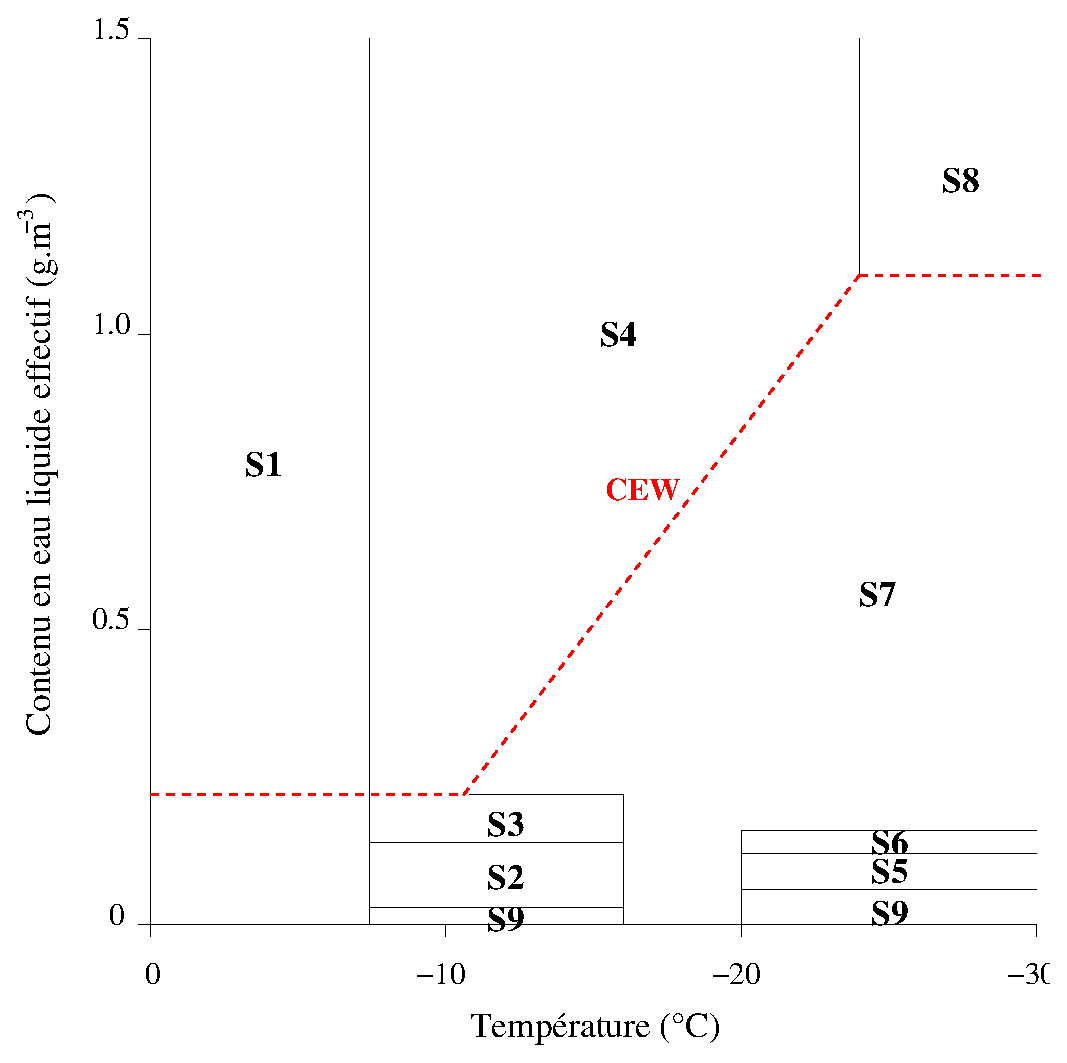
\includegraphics[width=8cm]{./EPS/saunders.eps}
  \end{center}
  \caption{\small Graphical representation of the regions of charge transfer as a function of temperature and effective liquid water content (\citet{Helsdon-2001} adapted from \citet{Saunders-1991}).}
  \label{fig:saunders}
\end{figure}
$EW$ is the effective liquid water content.
It is equal to the liquid water content times the drop collision efficiency. 
$EW$ is used instead of $LWC$ because the charge transfer mechanism is dependant on the rate of capture of the droplets rather than the liquid water content in the cloud.
The critical liquid water content, $CEW$, is defined as :
\begin{equation}
  CEW = -0.49 - 6.64 \times 10^{-2} T
\end{equation}
where $T$ is given in $^{\circ}$C.

\noindent
The equations describing each region of the graph are given in Table \ref{tab:eq_saund}.
\begin{table}[h]
  \begin{center}
  \begin{tabular}{|c|c|}
    \hline
    Equation number & Charge transfer equation\\
    \hline
    S1 & values linearly interpolated\\
    \hline
    S2 & $\delta Q = -314.40 \times EW + 7.92$\\
    \hline
    S3 & $\delta Q = 419.40 \times EW - 92.64$\\
    \hline
    S4 & $\delta Q = 20.22 \times EW + 1.36 \times T + 10.05$\\
    \hline
    S5 & $\delta Q = 2041.76  \times EW - 128.70$\\
    \hline
    S6 & $\delta Q = -2900.22 \times EW + 462.91$\\
    \hline
    S7 & $\delta Q = 3.02 - 31.76 \times EW + 26.53 \times EW^{2}$\\
    \hline
    S8 & $\delta Q = 20.22 \times EW - 22.26$\\
    \hline
    S9 & $\delta Q = 0.0$\\
    \hline
  \end{tabular}
  \end{center}
  \caption{\small Charge transfer equations from \citet{Saunders-1991}.}
  \label{tab:eq_saund}
\end{table}
In region S1, there is no laboratory results for temperature higher than -7.35$^{\circ}$C.
So, the values of $\delta Q$ at -7.35$^{\circ}$C are linearly interpolated until 0$^{\circ}$C.
At $T$ = 0$^{\circ}$C, the charge tranfer is null.
This interpolation concerns regions S1, S2, S3 and S9 :
\begin{equation}
  \begin{array}{lcl}
    \delta Q_{S1} & = & (-2.75 \times EW - 0.007) \times T \\
    \delta Q_{S3} & = & (-57.06 \times EW + 12.60) \times T \\
    \delta Q_{S2} & = & (42.78 \times EW - 1.08) \times T \\
    \delta Q_{S9} & = & 0
  \end{array}
\end{equation}

%--------------------------------------------------------
\subsubsection{Saunders and Peck (1998) parameterization}
%--------------------------------------------------------

\citet{Brooks-1997} reexamined the results of \citet{Saunders-1991} laboratory experiments, but transformed the effective liquid water content ($EW$) into the rime accretion rate ($RAR$, in g m$^{-2}$ s$^{-1}$):
$$RAR = EW \times V$$
with $V$ the relative velocity of the two particles ($x$ and $y$) experiencing collision.
In Meso-NH, the rime accretion rate is defined by:
\begin{equation}
  \begin{array}{rl}
    RAR = \rho _{air} \times r_c \times E_{cg} \times |V_{xmean} - V_{ymean}|  \mbox{ with } V_{mean} = \frac{\int _0 ^{+\infty} V(D) m(D) n(D) dD}{\int _0 ^{+\infty} m(D) n(D) dD}
  \end{array}
\end{equation}
$E_{cg}$ represents the collection efficiency of cloud droplets by graupel, and $V_{mean}$ is the mean fall speed of the considered particle.
The charge exchanged (in fC) during an elastic collision between two ice particles is the same as in the parameterization of \citet{Saunders-1991}:
\begin{equation}
  \delta q_{NI} ^{SP98} = B D ^m (\Delta v)^n \delta Q 
\end{equation}
$D$ is the diameter of the smallest particle (m), $\Delta v$ is the relative fall speed (m s$^{-1}$).
The $m$, $n$ and $B$ coefficients are the same as for \citet{Saunders-1991} (see Table \ref{tab:param_saund}).
The critical rime accretion rate ($RAR _{crit}$, in g m$^{-2}$ s$^{-1}$) is the RAR above which the biggest particle charges positively and below which it charges negatively:
\begin{equation}
  RAR_{crit} = a + b T + c T^2 + d T^3 + e T^4 + f T^5 + g T^6
\end{equation}
$a = 1.0$, $b = 7.9262 \times 10^{-2}$, $c = 4.4847 \times 10^{-2}$, $d = 7.4754 \times 10^{-3}$, $e = 5.4686 \times 10^{-4}$, $f = 1.6737 \times 10^{-5}$ et $g = 1.7613 \times 10^{-7}$.

\begin{figure}[h]
  \begin{center}
     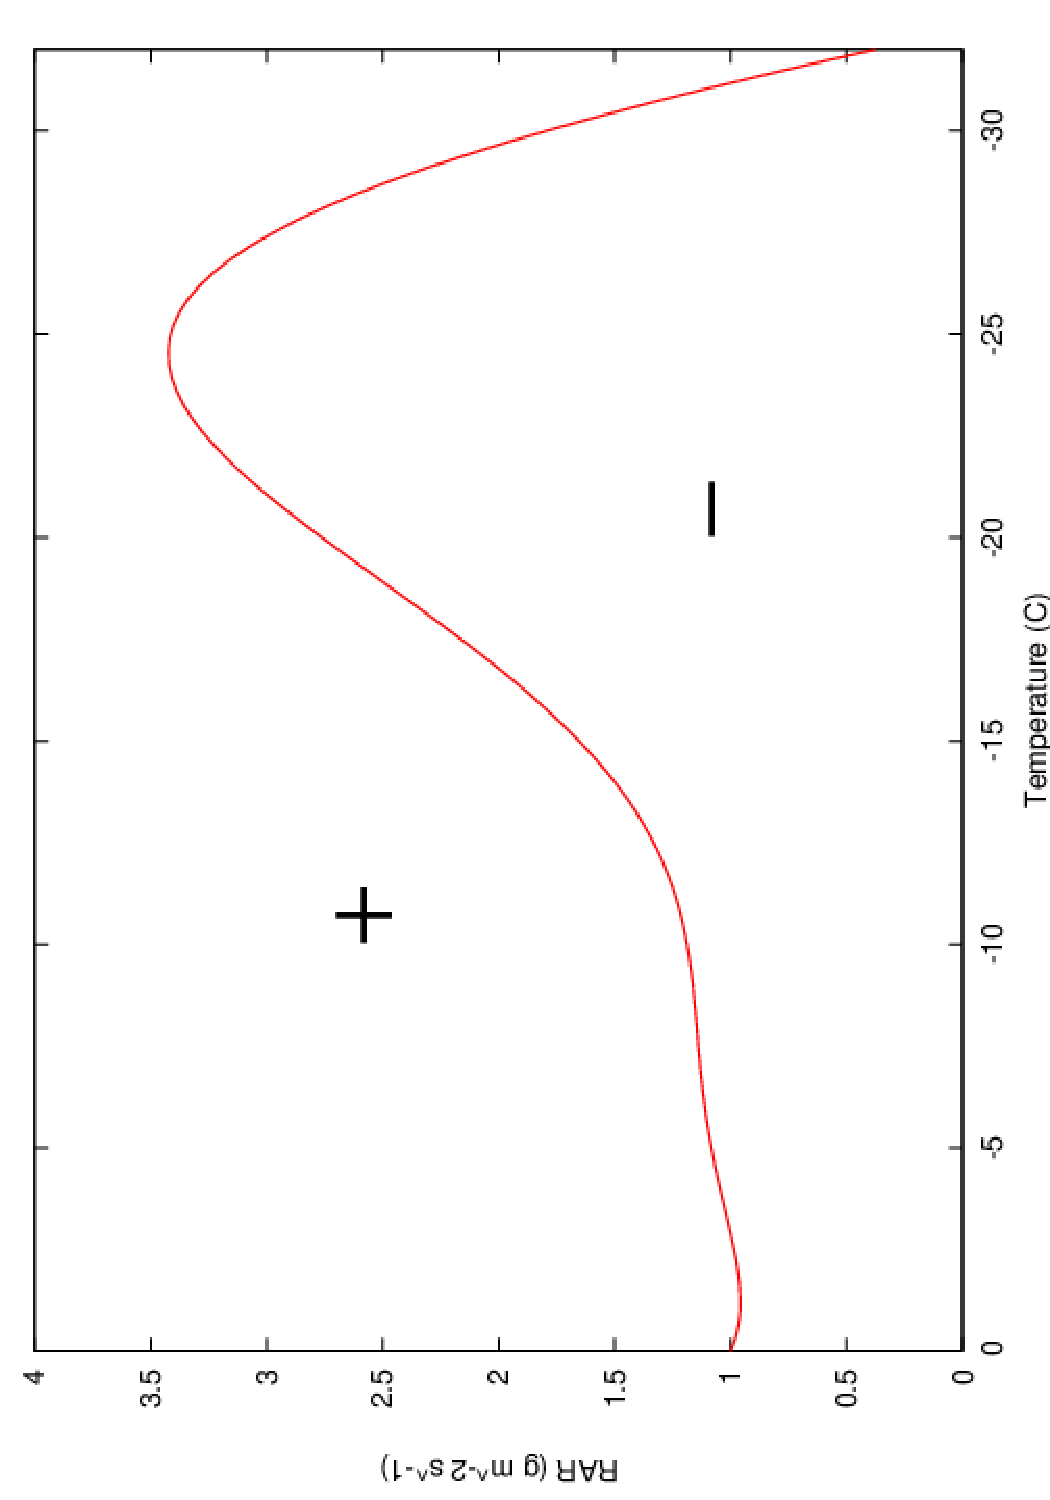
\includegraphics[angle=270,width=8cm]{./EPS/saunders_peck.pdf}
  \end{center}
  \caption{Plot of the critical rime accretion rate curve (red line) used in the \citet{Saunders-1998} noninductive ice-ice parameterization. Graupel charges positively at rime accretion rates above the curve and negatively below.}
  \label{fig:saunders_peck}
\end{figure}

The charge transfered per collision ($\delta Q$, in fC) depends on the temperature and the rime accretion rate.
Since the original equations of \citet{Saunders-1998} are only valid for temperatures between -8$^{\circ}$C and -23$^{\circ}$C, the parameterization of \citet{Saunders-1998} is adapted, partially following \citet{Mansell-2005}.

For $RAR < RAR_{crit}$, Equation (20) of \citet{Mansell-2005} is used to extend the application of the charge separation regime to $RAR$ between 0.1 and 0.3 g m$^{-2}$ s$^{-1}$. 
\begin{equation}
  \delta Q = 3.9 (RAR_{crit} - 0.1) \times \left( 4 \left[ \frac{RAR - (RAR_{crit} + 0.1)/2}{RAR_{crit} - 0.1}\right]^2 -1 \right)
\end{equation}

For $RAR > RAR_{crit}$, the original formula of \citet{Saunders-1998} is kept.
Outside the temperature range of -8$^{\circ}$C to -23$^{\circ}$C where the original \citet{Saunders-1998} scheme is strictly valid, the charging rate is linearly decreased to zero at 0(-40)$^{\circ}$C from the computed value at -8(-23)$^{\circ}$C, as suggested by \citet{Mansell-2005}.
Then for $RAR > RAR_{crit}$ and $T < -8^{\circ}$C:
\begin{equation}
  \delta Q = 6.74 RAR - 1.36 (-T) + 10.05
\end{equation}
while for $RAR > RAR_{crit}$ and $T > -8^{\circ}$C:
\begin{equation}
  \delta Q = -(6.74 RAR - 0.83) \times \frac{(T-T_t)}{8}
\end{equation}
Charging is set to 0 for $RAR < 0.1$ g m$^{-2}$ s$^{-1}$.

%----------------------------------------------------
\subsubsection{Brooks et al. (1997) parameterization}
%----------------------------------------------------

This parameterization uses the original parameterization of non-inductive charging proposed in \citet{Brooks-1997}, where the separated charge in \citet{Saunders-1991} is calculated by means the rime accretion rate $RAR$.
The critical liquid water content, $CRAR$, is defined as :
\begin{equation}
  CRAR = -1.47 - 0.2 \times T
\end{equation}

\noindent
The equations of \citet{Brooks-1997} describing each region of the graph are given in Table \ref{tab:eq_brook}.
\begin{table}[h]
  \begin{center}
  \begin{tabular}{|c|c|}
    \hline
    Equation number & Charge transfer equation\\
    \hline
    S1 & values linearly interpolated\\
    \hline
    S2 & $\delta Q = -104.8 \times RAR + 7.92$\\
    \hline
    S3 & $\delta Q = 139.8 \times RAR - 92.64$\\
    \hline
    S4 & $\delta Q = 6.74 \times RAR + 1.36 \times T + 10.05$\\
    \hline
    S5 & $\delta Q = 680.6  \times RAR - 128.70$\\
    \hline
    S6 & $\delta Q = -966.73 \times RAR + 462.91$\\
    \hline
    S7 & $\delta Q = 3.02 - 10.59 \times RAR + 10.59 \times RAR^{2}$\\
    \hline
    S8 & $\delta Q = 6.74 \times RAR - 22.26$\\
    \hline
    S9 & $\delta Q = 0.0$\\
    \hline
  \end{tabular}
  \end{center}
  \caption{\small Charge transfer equations from \citet{Brooks-1997}.}
  \label{tab:eq_brook}
\end{table}

The values of $\delta Q$ at -7.35$^{\circ}$C are linearly interpolated until 0$^{\circ}$C.
At $T$ = 0$^{\circ}$C, the charge transfer is null.
This interpolation concerns regions S1, S2, S3 and S9:
\begin{equation}
  \begin{array}{lcl}
    \delta Q_{S1} & = & (-0.9 \times RAR - 0.007) \times T \\
    \delta Q_{S3} & = & (-19.02 \times RAR + 12.60) \times T \\
    \delta Q_{S2} & = & (14.26 \times RAR - 1.08) \times T \\
    \delta Q_{S9} & = & 0
  \end{array}
\end{equation}

%-------------------------------------------------------------------------------------------------
\subsubsection{Tsenova and Mitzeva (2009) parameterization of Takahashi (1978) laboratory results}
%-------------------------------------------------------------------------------------------------

This parameterization uses the work of \citet{Tsenova-2009} where empirical equations for sign and magnitude of separated charge obtained by \citet{Takahashi-1978} are proposed. 
The sign and amplitude of the charge exchanged are expressed according to \citet{Saunders-1991}:
\begin{equation}
  \delta q_{NI} ^{T09} = B D_i ^m (\Delta v_{gi})^n \delta Q
\end{equation}

\noindent
The values of the constants $m$, $n$ and $B$ are given in Table \ref{tab:param_taka1}.
\begin{table}[h]
  \begin{center}
  \begin{tabular}{|c|c|c|c|c|}
    \hline
    Crystal size ($\mu$ m) & Situation & B & m & n \\
    \hline
    d $<$ 155            & + & 6.1  $\times$ 10$^{12}$ & 3.76 & 2.5 \\
    \hline
    155 $<$ d $\leq$ 452 & + & 5    $\times$ 10$^{5}$  & 1.90 & 2.5 \\
    \hline
    d $>$ 452            & + & 6.5                     & 0.44 & 2.5 \\
    \hline
    d $\leq$ 253         & - & 4.3  $\times$ 10$^{7}$  & 2.54 & 2.8 \\
    \hline
    d $>$ 253            & - & 2                       & 0.50 & 2.8 \\
    \hline
  \end{tabular}
  \end{center}
  \caption{\small Values of constants $B$, $m$ and $n$ proposed by \citet{Tsenova-2009} to be used in the equation of the charge transfer obtained in \citet{Takahashi-1978}.}
  \label{tab:param_taka1}
\end{table}

\noindent
(1) For $T$ $>$ -10$^{\circ}$C:
\begin{itemize}
  \item at $EW$ $<=$ 1.6 g m$^{-3}$:
\begin{eqnarray}
 \delta Q & = & 146.981 \times EW - 116.37 \times EW^{2} + 29.762 \times EW^{3}  \nonumber \\
          &   & - 0.03 \times T^{3} \times EW - 2.581 \times T - 0.0209 \times T^{3} \times EW^{3} \nonumber \\
          &   & + 0.356 \times T^{3} \times EW^{2} + 0.15 \times T^{2} + 2.918 \times T \times EW^{3} \nonumber  \\ 
          &   & - 4.215 \times T \times EW - 8.5059 
\end{eqnarray}
  \item at $EW$ $>$ 1.6 g m$^{-3}$:
\begin{eqnarray}
 \delta Q & = & 4.179 \times T - 0.0045 \times T^{2} \times EW^{2} + 0.916 \times EW^{2} \nonumber \\
          &   & - 1.333 \times T \times EW - 7.465 \times EW + 0.109 \times T \times EW^{2} \nonumber \\
          &   & + 0.0006 \times T^{2} \times EW^{3} - 0.035 \times EW^{3} + 50.845
\end{eqnarray}
\end{itemize}

\noindent
(2) For $T$ $<=$ -10$^{\circ}$C:
\begin{itemize}
  \item at $EW$ $<=$ 0.4 g m$^{-3}$:
\begin{eqnarray}
 \delta Q & = & -3.35 \times T + 95.9 \times T \times EW^{2} + 511.83 \times EW \nonumber \\
          & + & 17.45 \times T^{2} \times EW^{3} - 0.0007 \times T^{3} + 20.57 \times T \times EW \nonumber \\
          &   & + 0.165 \times T^{2} \times EW + 0.495 \times T^{3} \times EW^{3} - 0.098 \times T^{3} \times EW^{2} \nonumber  \\
          &   & +67.46 \times T \times EW^{3} - 0.107 \times T^{2} - 24.5715
\end{eqnarray}
  \item at 0.4 g m$^{-3}$ $<$ $EW$ $<=$ 3.2 g m$^{-3}$:
\begin{eqnarray}
 \delta Q & = & -1.567 \times T \times EW + 0.248 \times T \times EW^{3} + 0.01 \times T^{3} \nonumber \\
          &   & + 19.2 \times T + 0.805 \times T^{2} + 5.97 \times EW^{3} - 83.39 \times EW \nonumber \\
          &   & + 15.36 \times EW^{2} + 167.93
\end{eqnarray}
  \item at $EW$ $>$ 3.2 g m$^{-3}$:
\begin{equation}
 \delta Q = 4.213 \times T - 0.831 \times T \times EW + 0.067 \times T \times EW^{2} + 0.004 \times T^{2} \times EW + 40.964
\end{equation}
\end{itemize}

%-------------------------------------------------------------------------------------------------
\subsubsection{Tsenova and Mitzeva (2011) parameterization of Takahashi (1978) laboratory results}
%-------------------------------------------------------------------------------------------------

This parameterization uses the work of \citet{Tsenova-2011} where empirical equations for sign and magnitude of separated charge obtained by \citet{Takahashi-1978} using the rime accretion rate ($RAR$) are proposed.

\noindent
(1) For $T$ $>$ -10$^{\circ}$C:
\begin{itemize}
  \item at $RAR$ $<=$ 12.8 g m$^{-2}$ s$^{-1}$:
\begin{eqnarray}
 \delta Q & = & 18.37 \times RAR - 1.82 \times RAR^{2} - 0.06 \times RAR^{3} \nonumber \\
          &   & - 0.004 \times T^{3} \times RAR - 2.581 \times T + 0.0004 \times T^{3} \times RAR^{3} \nonumber \\
          &   & + 0.006 \times T^{3} \times RAR^{2} + 0.15 \times T^{2} + 0.006 \times T \times RAR^{3} \nonumber \\ 
          &   & - 0.53 \times T \times RAR - 8.5059 
\end{eqnarray}
  \item at $RAR$ $>$ 12.8 g m$^{-2}$ s$^{-1}$:
\begin{eqnarray}
 \delta Q & = & 4.179 \times T - 0.00007 \times T^{2} \times RAR^{2} + 0.01 \times RAR^{2} \nonumber \\
          &   & - 0.17 \times T \times RAR - 0.93 \times RAR + 0.002 \times T \times RAR^{2} \nonumber \\
          &   & + 0.000001 \times T^{2} \times RAR^{3} - 0.00007 \times RAR^{3} + 50.845
\end{eqnarray}
\end{itemize}

\noindent
(2) For $T$ $<=$ -10$^{\circ}$C:
\begin{itemize}
  \item at $RAR$ $<=$ 3.2 g m$^{-2}$ s$^{-1}$:
\begin{eqnarray}
 \delta Q & = & -3.35 \times T + 1.5 \times T \times RAR^{2} + 63.98 \times RAR \nonumber \\
          &   & + 0.03 \times T^{2} \times RAR^{3} - 0.0007 \times T^{3} + 2.57 \times T \times RAR \nonumber \\
          &   & + 0.02 \times T^{2} \times RAR + 0.001 \times T^{3} \times RAR^{3} - 0.002 \times T^{3} \times RAR^{2} \nonumber \\
          &   & + 0.13 \times T \times RAR^{3} - 0.107 \times T^{2} - 24.5715
\end{eqnarray}
  \item at 3.2 g m$^{-2}$ s$^{-1}$ $<$ $RAR$ $<=$ 25.6 g m$^{-2}$ s$^{-1}$:
\begin{eqnarray}
 \delta Q & = & -0.2 \times T \times RAR + 0.0005 \times T \times RAR^{3} + 0.01 \times T^{3} \nonumber \\
          &   & + 19.2 \times T + 0.805 \times T^{2} + 0.01 \times RAR^{3} - 10.42 \times RAR \nonumber \\
          &   & + 0.24 \times RAR^{2} + 167.93
\end{eqnarray}
  \item at $RAR$ $>$ 25.6 g m$^{-2}$ s$^{-1}$:
\begin{equation}
 \delta Q = 4.213 \times T - 0.1 \times T \times RAR + 0.001 \times T \times RAR^{2} + 0.0005 \times T^{2} \times RAR + 40.964
\end{equation}
\end{itemize}


\paragraph{Limitations of the charge exchanged per collision}

As in \citet{Mansell-2005}, the charge exchanged per rebounding collision $\delta q$ is limited to prevent unreasonable charging rate.
Based on \citet{Keith-1990}, it is assumed that the charging rate of the pristine ice crystal with $D_{max}$ $\sim$ 100 $\mu$m is the most limiting one, that is 30(10) fC per collision with graupel(aggregate) particles.
We take a larger value (100 fC) for the graupel-snow collisions because it corresponds roughly to an average of the saturation levels when the particle sizes reach $\sim$ 1 mm (see \citet{Keith-1990} or Fig. 3.13 in \citet{MacGorman-Rust}).
This limitation is introduced in the computation of the bulk charging rates which result from an integration over the size spectrum of the ice particles.


%++++++++++++++++++++++++++++++++
\subsection{Inductive mechanism}
%++++++++++++++++++++++++++++++++

Laboratory studies conducted by \citet{Aufdermaur-1972} have shown that in the presence of an electric field stronger than a few kV m$^{-1}$ collisions between particles would lead to significant charge exchange. 
Drop-drop inductive charging is not considered because most of the time the two colliding particles end up with a single bigger drop. 
Concerning ice-ice inductive charging, the short duration and small size of the contact zone and the low ice electrical conductivity do not allow for a substantial charge exchange when ice particles collide \citep{Illingworth-1985a}. 
Therefore only bouncing collisions between graupel and droplets are likely needed to be taken into account. 
Even if the rate of rebounding collisions is low compared to the rate of sticking collisions, the amount of charge separated is important. 
The inductive charging rate parameterization follows the expression given by \citet{Ziegler-1991}:
\begin{equation}
  \frac{\partial \rho_g (D_g)}{\partial t} = \frac{\pi}{4} E_{cg} E_r D_g ^2 V(D_g) N_c \alpha \left[ \frac{\pi ^3}{2} D_c ^2 \epsilon E_z \cos(\theta) - \frac{\pi ^2}{6}\rho_g(D_g) \frac{D_c ^2}{D_g ^2} \right]
\end{equation}
where $E_{cg}$ is the graupel-droplets collision efficiency, $E_r$ the rebound probability, and $E_z$ the vertical component of the electric field. 
$\epsilon$ is the permittivity of air. 
$\rho _g$ is the graupel charge density, $D_c$ the cloud droplets diameter, and $D_g$ the graupel diameter. 
$V$ is the fall speed of graupel, and $N_c$ is the number concentration of cloud droplets. 
The second term of the expression accounts for a preexisting charge polarity of the graupel. 
Assuming that grazing collisions are the most efficient ones, $\alpha$ is the fraction of droplets experiencing grazing trajectories, and $\cos(\theta)$ is the mean cosine collision angle. 
$E_r$, $\alpha$ and $\cos(\theta)$ are set to 0.1, 0.07 and 0.2, respectively, as suggested by \citet{Ziegler-1991}.


%%%%%%%%%%%%%%%%%%%%%%%%%%%%%%%%%%%%%%%%%%%%%%%%%%%%%%%
\section{Charge transfers associated to mass transfers}
\label{sec:micro}
%%%%%%%%%%%%%%%%%%%%%%%%%%%%%%%%%%%%%%%%%%%%%%%%%%%%%%%

Once charges are separated by the non-inductive process, they can be exchanged between the different hydrometeor categories during the microphysical processes.

\begin{figure}[h]
  \begin{center}
     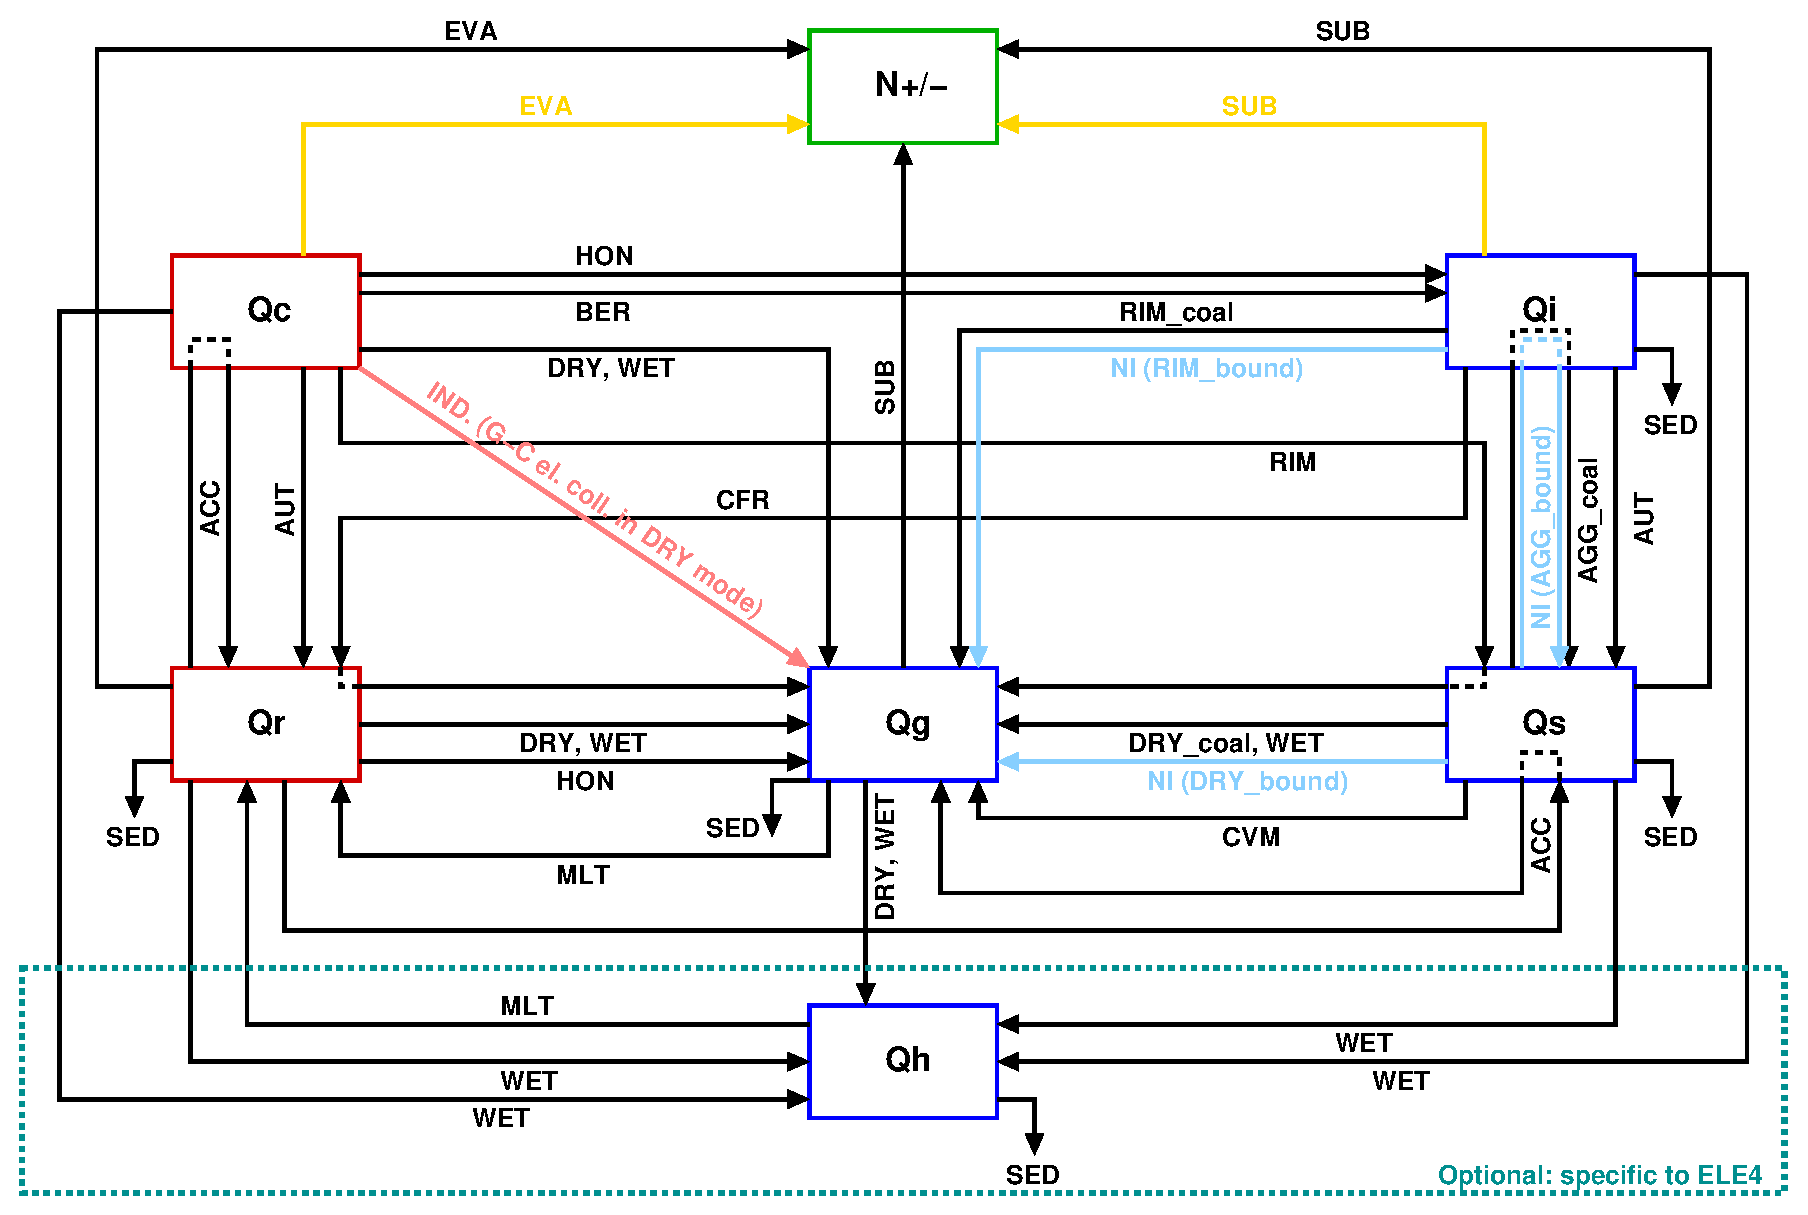
\includegraphics[width=16cm]{./EPS/charge_transfer.eps}
  \end{center}
  \caption{Diagram of the electric charge transfers. Black, light blue and pink lines represent charge transfers associated to mass transfers, to the non-inductive mechanisms, and to the inductive mechanism, respectively. The yellow lines show the electric charge transfers treated as an ajustement in ice\_adjust\_elec.f90. Ion attachment to hydrometeors is not represented in this diagram.}
  \label{fig:transfer}
\end{figure}

Similarly to the microphysical scheme, the rate of charge exchanged during mass transfer follows:
\begin{equation}
  QYCOLXZ = \int_0 ^{+ \infty} \left\{
            \int_0 ^{+ \infty} K(D_x , D_y) q_y n_y (D_y) dD_y \right\} n_x (D_x) dD_x
\end{equation}
The kernel $K$ can be written:
\begin{equation}
  K(D_x , D_y) = \frac{\pi}{4} (D_x + D_y)^2 |v_x (D_x) - v_y (D_y)| E_{xy}
\end{equation}
$E_{xy}$ is the collection efficiency.

%+++++++++++++++++++++++++
\subsection{Sedimentation}
%+++++++++++++++++++++++++

For precipitating particles (rain, snow, graupel and hail, then X = R, S, G and H), the sedimentation rate of charge density follows:
\begin{equation}
  QSEDX = \frac{\partial}{\partial z} \left[ \left( \frac{\rho _{00}}{\rho _{dref}} \right) ^{0.4} c_x e_x C_x G(d_x + f_x) \lambda ^{x - (d_x + f_x)} \right]
\end{equation}
For pristine ice:
\begin{equation}
  QSEDI = \frac{\partial}{\partial z} \left[ \left( \frac{\rho _{00}}{\rho _{dref}} \right) ^{0.4} c_i e_i N_i G(d_i + f_i) \left( \frac{\rho _{dref} r_i}{a_i N_i G(b_i)} \right) ^{\frac{d_x + f_x}{b_x}} \right]
\end{equation}

%++++++++++++++++++++++++++
\subsection{Warm processes}
%++++++++++++++++++++++++++

\paragraph{Autoconversion}

\begin{equation}
  QCAUTR = q_c \frac{RCAUTR}{r_c}
\end{equation}


\paragraph{Accretion}

\begin{equation}
  QCACCR = q_c \frac{RCACCR}{r_c}
\end{equation}


\paragraph{Evaporation and condensation of rain}

\begin{equation}
  QREVAV = q_r \frac{RREVAV}{r_r} 
\end{equation}
The charge released during rain evaporation is transfered to the ions categories following:
\begin{eqnarray}
  n_+ &=& n_+ + QREVAV / e \quad {\rm if} \quad QREVAV > 0 \\
  n_- &=& n_- - QREVAV / e \quad {\rm if} \quad QREVAV < 0
\end{eqnarray}

%++++++++++++++++++++++++++
\subsection{Ice nucleation}
%++++++++++++++++++++++++++

\paragraph{Heterogeneous nucleation}

It is considered there is no charge exchanged during this mass transfer.


\paragraph{Homogeneous nucleation}

For temperatures colder than -35$^{\circ}$C, cloud droplets spontaneously freeze and are transfered to the ice crystals category.
If $P \approx J_{HOM}(T) V \Delta t$ is the probability for a cloud droplet with volume $V$ to freeze during $\Delta$t, the charge exchanged during this process can be computed in the same manner as for the microphysical process:
\begin{eqnarray}
  QCHONI & = & \int_0 ^{+ \infty} q_c P M_c (D_c) dD_c \nonumber \\
         & = & \frac{\pi}{6} J_{HOM} \rho r_c \frac{e_c}{a_c} \frac{G(f_c + 3)}{G(b_c)} \lambda ^{b_c - (f_c + 3)}
\end{eqnarray}
a$_{c}$ is the proportionality factor in the mass-diameter relation ($a_c = 1000 \times \frac{\pi}{6}$). 
Moments are computed using: $\lambda _{c}$ = 1.1 $\times$ 10$^{5}$ m$^{-3}$, $\alpha _{c}$ = 3 and $\nu _{c}$ = 1.


\paragraph{Homogeneous nucleation}

For temperatures lower than -35$^{\circ}$C, raindrops freeze spontaneously.
\begin{eqnarray}
  QRHONG & = & q_r H(T_t - 35) \nonumber \\
         & = & q_r \frac{RRHONG}{r_r}
\end{eqnarray}

%+++++++++++++++++++++++++++++++++++++
\subsection{Bergeron-Findeisen effect}
%+++++++++++++++++++++++++++++++++++++

\begin{equation}
  QCBERI = q_c \frac{RCBERI}{r_c}
\end{equation}
However, the charge exchanged during this process is too high.
Then QCBERI is reduced to 1\% of its value.

%++++++++++++++++++++++++++++++++++++++++++++++++++++++
\subsection{Water vapor deposition on snow and graupel}
%++++++++++++++++++++++++++++++++++++++++++++++++++++++

\begin{eqnarray}
  QSSUBV &=& q_s \frac{RSSUBV}{r_s} \\
  QGSUBV &=& q_g \frac{RGSUBV}{r_g}
\end{eqnarray}
RSSUBV and RGSUBV are the negative part of the mass transfer rate during vapor deposition.

The charge released during the graupel/snow ($x = G/S$) sublimation is transfered to the ions categories following:
\begin{eqnarray}
  n_+ &=& n_+ + \frac{QxSUBV}{e}  \mbox{ if } QxSUBV > 0 \\
  n_- &=& n_- - \frac{QxSUBV}{e}  \mbox{ if } QxSUBV < 0
\end{eqnarray}

%++++++++++++++++++++++++++++++++++++++++++++++++++++++++++++++++
\subsection{Autoconversion of pristine ice and formation of snow}
%++++++++++++++++++++++++++++++++++++++++++++++++++++++++++++++++

\begin{equation}
  QIAUTS = q_i \frac{RIAUTS}{r_i}
\end{equation}

%+++++++++++++++++++++++++++++++++++++++++++++++++++++++++++++
\subsection{Contact freezing of rain and formation of graupel}
%+++++++++++++++++++++++++++++++++++++++++++++++++++++++++++++

This is a 3-species mechanism.
The collision between ice crystal and raindrop produces frozen drops.
If the pristine ice fall speed can be neglected compared to the raindrop fall speed, then the charge lost by raindrops is:
\begin{eqnarray}
  QRCFRIG &=& \int_0 ^{+ \infty} \left[ \int_0 ^{+ \infty}
    K(D_r , D_i) n_r (D_r) q_r (D_r) dD_r \right] n_i (D_i) dD_i \nonumber \\
          &=& \frac{\pi}{4} C_r N_i c_r e_r
              \left( \frac{\rho _{00}}{\rho _{dref}} \right) ^{0.4}
              G_r (d_r + f_r + 2) \lambda _r ^{x_r - (d_r + f_r + 2)}
\end{eqnarray}
And the charge lost by pristine ice is:
\begin{eqnarray}
  QICFRRG &=& \int_0 ^{+ \infty} \left[ \int_0 ^{+ \infty}
    K(D_r , D_i) n_i (D_i) q_i (D_i) dD_i \right] n_r (D_r) dD_r \nonumber \\
          &=& q_i \frac{\pi}{4} C_r \lambda _r ^{x_r} c_r
              \left( \frac{\rho _{00}}{\rho _{dref}} \right) ^{0.4}
              G_r (d_r + 2) \lambda _r ^{d_r + 2} \nonumber \\
          &=& q_i \frac{RICFRRG}{r_i}
\end{eqnarray}

%+++++++++++++++++++++++++++++++++++++++++++++++
\subsection{Aggregation of pristine ice on snow}
%+++++++++++++++++++++++++++++++++++++++++++++++

\begin{equation}
  QIAGGS = QIAGGS_{bound} + QIAGGS_{coal}
\end{equation}


\paragraph{Case with coalescence}

\begin{equation}
  QIAGGS_{coal} = \int_0 ^{+ \infty} \left\{\int_0 ^{+ \infty} \frac{\pi}{4} (D_i + D_s)^2 |v_i (D_i) - v_s (D_s)| E_{is} q_i n_i (D_i) dD_i \right\} n_s (D_s) dD_s \nonumber
\end{equation}
The ice-snow collection efficiency takes the form: $E_{is} = 0.25 \exp[0.005(T - T_t)]$.
The pristine ice diameter (fall speed) can be neglected compared to the snow diameter (fall speed):
\begin{eqnarray}
  QIAGGS_{coal} &=& \int_0 ^{+ \infty} \left\{\int_0 ^{+ \infty} \frac{\pi}{4} D_s^2 v_s (D_s) E_{is} q_i n_i (D_i) dD_i \right\} n_s (D_s) dD_s \nonumber \\
                &=& q_i \frac{RIAGGS}{r_i}
\end{eqnarray}


\paragraph{Case with elastic collision}

If ice crystals and snow particles experience elastic collisions, this is considered as part of the non-inductive mechanism.
The same approximations about diameter and fall speed as in the case with coalescence can be done.
\begin{eqnarray}
  QIAGGS_{boun} &=& \int_0 ^{+ \infty} \left\{\int_0 ^{+ \infty} \frac{\pi}{4} (D_i + D_s)^2 |v_i (D_i) - v_s (D_s)| (1 - E_{is}) q_i n_i (D_i) dD_i \right\} n_s (D_s) dD_s \nonumber \\
                &=& \frac{\pi}{4} (1 - E_{is}) c_s \left( \frac{\rho _{00}}{\rho _{dref}} \right) ^{0.4}
			\int_0 ^{+ \infty} D_s ^{(2 + d_s)} \left[ \int_0 ^{+ \infty} q_i n_i (D_i) dD_i \right] n_s (D_s) dD_s
\end{eqnarray}
Different parameterizations are available for this process.\\

\begin{enumerate}
  \item {\bf \textsc{Helsdon and Farley (1987)}}

For a snow-ice collision, $\delta q_{is} = 2.10^{-15}$C, then:
\begin{eqnarray}
  QIAGGS_{boun} &=& \frac{\pi}{4} (1 - E_{is}) c_s
                \left( \frac{\rho _{00}}{\rho _{dref}} \right) ^{0.4}
                \delta q_{is} N_i
                \int_0 ^{+ \infty} D_s ^{(2 + d_s)}  n_s (D_s) dD_s 
                \nonumber \\
                &=& \frac{1 - E_{is}}{E_{is}} RIAGGS 
                \frac{\delta q_{is}}{r_i} N_i
\end{eqnarray}

 \item {\bf\textsc{Takahashi (1978)}}

\begin{eqnarray}
  QIAGGS_{boun} &=& \frac{\pi}{4} (1 - E_{is}) c_s
                \left( \frac{\rho _{00}}{\rho _{dref}} \right) ^{0.4}
                \int_0 ^{+ \infty} D_s ^{(2 + d_s)}
                \left[ \int_0 ^{+ \infty} f(T,LWC) \times \right. \nonumber \\
                & & \left. {\rm Min} \left( 10, 5
                    \left( \frac{D_i}{D_0} \right) ^2
                    \frac{|v_s - v_i|}{v_0} \right) n_i (D_i) dD_i \right]
                n_s (D_s) dD_s \nonumber
\end{eqnarray}
It is assumed that $v_i \ll v_s$:
\begin{eqnarray}
  QIAGGS_{boun} &=& \frac{\pi}{4} (1 - E_{is}) c_s
                \left( \frac{\rho _{00}}{\rho _{dref}} \right) ^{0.4}
                f(T,LWC)
                \int_0 ^{+ \infty} D_s ^{(2 + d_s)}
                \left[ \int_0 ^{+ \infty} \times \right. \nonumber \\
                & & \left. {\rm Min} \left( 10, 5
                    \left( \frac{D_i}{D_0} \right) ^2
                    \frac{|v_s - v_i|}{v_0} \right) N_i g(D_i) dD_i \right]
                n_s (D_s) dD_s  \nonumber \\
                &=& \frac{\pi}{4} (1 - E_{is}) 
                \left( \frac{\rho _{00}}{\rho _{dref}} \right) ^{0.4}
                c_s N_i N_s f(T,LWC) \times \nonumber \\ 
                & & {\rm Min} \left[ 10 G_s (2 + d_s) \lambda _s ^{-(2 + d_s)},
                  \frac{5 c_s}{D_0 ^2 v_0} 
                  \left( \frac{\rho _{00}}{\rho _{dref}} \right) ^{0.4}
                  G_i (2) \lambda _i ^{-2} G_s (2 + 2d_s)
                  \lambda ^{-(2 + 2d_s)} \right] \nonumber \\
\end{eqnarray}

  \item {\bf \textsc{Gardiner et al. (1985)}}

\begin{eqnarray}
  QIAGGS_{boun} &=& \frac{\pi}{4} (1 - E_{is}) c_s
                \left( \frac{\rho _{00}}{\rho _{dref}} \right) ^{0.4}
                \int_0 ^{+ \infty} D_s ^{(2 + d_s)} \nonumber \\
                & & \left[ \int_0 ^{+ \infty} 73 D_i ^4 (v_s - v_i)^3
                  \delta L f(\tau) n_i (D_i) dD_i \right]
                n_s (D_s) dD_s \nonumber
\end{eqnarray}
Since $v_i \ll v_s$ :
\begin{equation}
  QIAGGS_{boun} = \frac{\pi}{4} (1 - E_{is})
                \left( \frac{\rho _{00}}{\rho _{dref}} \right) ^{4 \times 0.4}
                c_s ^4 N_i C_s G_i (4) \lambda _i ^{-4}
                G_s (2 + 4d_s) \lambda _s ^{x_s - (2 + 4d_s)}
                73 \delta L f(\tau) \times 10^{15}
\end{equation}

  \item {\bf \textsc{Saunders et al. (1991), Saunders et Peck (1998), Brooks et al. (1997), Tsenova and Mitzeva (2009, 2011)}}

\begin{eqnarray}
  QIAGGS_{boun} &=& \frac{\pi}{4} (1 - E_{is}) c_s
                \left( \frac{\rho _{00}}{\rho _{dref}} \right) ^{0.4}
                \int_0 ^{+ \infty} D_s ^{(2 + d_s)} \nonumber \\
                & & \left[ \int_0 ^{+ \infty} B D_i ^a |v_s - v_i | ^b \delta Q
                  N_i g(D_i) dD_i \right] n_s (D_s) dD_s \nonumber
\end{eqnarray}
$v_i \ll v_s$ and $q$ only depends on temperature and liquid water content:
\begin{eqnarray}
  QIAGGS_{boun} &=& \frac{\pi}{4} (1 - E_{is}) 
                  \left( \frac{\rho _{00}}{\rho _{dref}} \right)^{0.4(1 + b_s)}
                  c_s ^{1 + b_s} N_i C_s G_i (a_i) \lambda _i ^{a_i}
                  \nonumber \\
                & & G_s (2 + (1 + b_s) d_s ) 
                  \lambda _s ^{x_s - 2 - (1 + b_s)d_s} B \delta Q
\end{eqnarray}

\end{enumerate}

%++++++++++++++++++++++++++++++++
\subsection{Riming of aggregates}
%++++++++++++++++++++++++++++++++

During the riming of aggregates, cloud droplets lose charge at rate:
\begin{eqnarray}
  QCRIMS &=& \int_0 ^{+ \infty} \left[ \int_0 ^{+ \infty}
             \frac{\pi}{4} (D_s + D_c)^2 |v_s - v_c| E_{cs} q_c n_c (D_c) dD_c
             \right] n_s (D_s) dD_s \nonumber \\
         &=& q_c \frac{RCRIMS}{r_c}
\end{eqnarray}
We assume: $v_i \ll v_s$, $D_i \ll D_s$, and $E_{cs}$ = 1.
It is also hypothesized that conversion of aggregates into graupels may occur for riming aggregates of size larger than $D_{cs} ^{lim}$ = 7 mm \citep{Farley-1989}.
Thus the charge gained by aggregates during their growth by riming takes the form:
\begin{eqnarray}
  QCRIMSS &=& \int_0 ^{D_s ^{lim}} \left[ \int_0 ^{+ \infty}
              \frac{\pi}{4} (D_s + D_c)^2 |v_s - v_c| E_{cs} q_c n_c (D_c) dD_c
              \right] n_s (D_s) dD_s \nonumber \\
          &=& \frac{\pi}{4} 
              \left( \frac{\rho _{00}}{\rho _{dref}} \right)^{0.4}
              c_s C_s \lambda ^{x_s} q_c M(S + d_s ; D_s ^{lim}) \nonumber \\
          &=& q_c \frac{RCRIMSS}{r_c}
\end{eqnarray}
If $D_s > D_{cs} ^{lim}$:
\begin{eqnarray}
  QCRIMSG &=& \int_0 ^{+ \infty} \left[ \int_{D_s ^{lim}} ^{+ \infty}
              \frac{\pi}{4} (D_s + D_c)^2 |v_s - v_c| E_{cs} q_c n_c (D_c) dD_c
              \right] n_s (D_s) dD_s \nonumber \\
          &=& QCRIMS - QCRIMSS \nonumber \\
          &=& \frac{q_c}{r_c} (RCRIMS - RCRIMSS)
\end{eqnarray}

%++++++++++++++++++++++++++++++++++++++++++++
\subsection{Accretion of rain and aggregates}
%++++++++++++++++++++++++++++++++++++++++++++

As for the riming of cloud droplets, it is postulated that the collection of small raindrops do not change the structure of an aggregate but larger colliding raindrops reshape it as a graupel.
The rate of charge exchanged during the collection of raindrops by snow has the form:
\begin{equation}
  QRACCS = \int_0 ^{+ \infty} \left[ \int_0 ^{+ \infty}
           \frac{\pi}{4} (D_s + D_r)^2 |v_r - v_s| E_{rs} q_r n_r (D_r) dD_r
           \right] n_s (D_s) dD_s \nonumber
\end{equation}
It is assumed that $E_{rs}$ = 1.
Furthermore, as both raindrops and aggregates have significant fall speeds, it is not easy to solve the integrals.
They are tabulated in function of $\lambda _{r}$ et $\lambda _{s}$.
\begin{eqnarray}
  QRACCS & = & \int_0 ^{+ \infty} \left[ \int_0 ^{+ \infty}
           E_{rs} \frac{\pi}{4} 
           \left( \frac{\rho _{00}}{\rho _{dref}} \right)^{0.4}
           (D_r + D_s)^2 |c_r D_r ^{d_r} - c_s D_s ^{d_s}| q_r N_r g(D_r) dD_r
           \right] \times \nonumber \\
         &   & N_s g(D_s) dD_s \nonumber
\end{eqnarray}
We define:
\begin{eqnarray}
  \Delta vq_{rs}(\lambda _s, \lambda _r) & = &
    \Lambda q(\lambda _s, \lambda _r)^{-1} \int_0 ^{+ \infty} \left[
      \int_0 ^{+ \infty} E_{rs} (D_r + D_s)^2 
      |c_r D_r ^{d_r} - c_s D_s ^{d_s}| D_r ^{f_r} g(D_r , \lambda _r)dD_r 
    \right] \times \nonumber \\
                                         &   & g(D_s , \lambda _s) dD_s \nonumber
\end{eqnarray}
with:
\begin{eqnarray}
  \Lambda q(\lambda _s, \lambda _r) &=& \int_0 ^{+ \infty} \left[ 
    \int_0 ^{+ \infty} (D_r + D_s)^2 D_r ^{f_r} g(D_r , \lambda _r) dD_r
    \right] g(D_s , \lambda _s) dD_s \nonumber \\
   &=& M_r(2 + f_r) + M_s(2)M(f_r) + 2 M_s(1) M_r(1 + f_r) \nonumber \\
   &=& G_r(2 + f_r) \lambda _r ^{-(2 + f_r)} + G_s(2) G(f_r) \lambda _s ^{-2} 
       \lambda _r ^{-f_r} \nonumber \\
   & & + 2 G_s(1) G_r(1 + f_r) \lambda _s ^{-1} 
       \lambda _r ^{-(1+f_r)} 
\end{eqnarray}
Since $q_r (D_r) = e_r D_r ^{f_r}$:
\begin{equation}
  QRACCS = \frac{\pi}{4} \left( \frac{\rho _{00}}{\rho _{dref}} \right)^{0.4}
           N_r N_s e_r \Delta vq_{rs}(\lambda _s, \lambda _r)
           \Lambda q(\lambda _s, \lambda _r)
\end{equation}

\noindent
\underline{If $D_r < D_{r} ^{lim}$}, the structure of the aggregates is not changed:
\begin{eqnarray}
  QRACCSS &=& \int_0 ^{+ \infty} \left[ \int_0 ^{D_r ^{lim}}
            \frac{\pi}{4} (D_r + D_s)^2 |v_r - v_s| E_{rs} q_r (D_r) 
            n_r (D_r) dD_r
            \right] n_s (D_s) dD_s \nonumber \\
          &=& \frac{\pi}{4} 
              \left( \frac{\rho _{00}}{\rho _{dref}} \right)^{0.4}
              N_s N_r e_r \Lambda q(\lambda _s, \lambda _r)
              \Delta vq_{rss}(\lambda _s, \lambda _r)
\end{eqnarray}
with :
\begin{eqnarray}
  \Delta vq_{rss}(\lambda _s, \lambda _r) & = &
    \Lambda q(\lambda _s, \lambda _r)^{-1} \int_0 ^{+ \infty} \left[
      \int_0 ^{D_r ^{lim}} E_{rs} (D_r + D_s)^2 
      |c_r D_r ^{d_r} - c_s D_s ^{d_s}| D_r ^{f_r} g(D_r , \lambda _r)dD_r 
    \right] \times \nonumber \\
      &  & g(D_s , \lambda _s) dD_s
\end{eqnarray}

\noindent
\underline{If $D_r > D_{r} ^{lim}$}, the structure of the aggregates is turned into graupel.
The rate of charge transfered from rain to graupel is:
\begin{equation}
  QRACCSG = QRACCS - QRACCSS
\end{equation}
Since $q_x (D_x) = e_x D_x ^{f_x}$, $n_x (D_x) = N_x g(D_x) = C_x \lambda ^{x_x} g(D_x)$ and $v_{x}(D_x) =  \left( \frac{\rho _{00}}{\rho _{dref}} \right)^{0.4} c_x D_x ^{d_x}$, with $x$ = $r$ or $s$, the charge lost by aggregates follows:
\begin{eqnarray}
  QSACCRG &=& \int_{D_r ^{lim}} ^{+ \infty} \left[ \int_0 ^{+ \infty} 
              \frac{\pi}{4} E_{rs} (D_r + D_s)^2 |v_r (D_r) - v_s (D_s)|
              q_s (D_s) n_s (D_s) dD_s \right] n_r (D_r) dD_r \nonumber \\
          &=& \frac{\pi}{4} 
              \left( \frac{\rho _{00}}{\rho _{dref}} \right)^{0.4}
              N_s N_r e_s
              \Lambda q(\lambda _s, \lambda _r)
              \Delta vq_{rs}(\lambda _s, \lambda _r)
\end{eqnarray}
with:
\begin{eqnarray}
  \Delta vq_{rss}(\lambda _s, \lambda _r) & = &
    \Lambda q(\lambda _s, \lambda _r)^{-1} \int_{D_r ^{lim}} ^{+ \infty}
    \left[ \int_0 ^{+ \infty}  E_{rs} (D_r + D_s)^2 
       |c_r D_r ^{d_r} - c_s D_s ^{d_s}| D_s ^{f_s}  g(D_s , \lambda _s) dD_s
       \right] \times \nonumber \\
       &  & g(D_r , \lambda _r)dD_r 
\end{eqnarray}
\begin{eqnarray}
  \Lambda q(\lambda _s, \lambda _r) &=& \int_0 ^{+ \infty} \left[ 
    \int_0 ^{+ \infty} (D_r + D_s)^2 D_s ^{f_s} g(D_s , \lambda _s) dD_s
    \right] g(D_r , \lambda _r) dD_r \nonumber \\
   &=& M_s(2 + f_s) + M_r(2)M(f_s) + 2 M_r(1) M_s(1 + f_s) \nonumber \\
   &=& G_s(2 + f_s) \lambda _s ^{-(2 + f_s)} + G_r(2) G(f_s) \lambda _r ^{-2} 
       \lambda _s ^{-f_s} \nonumber \\
   & & + 2 G_r(1) G_s(1 + f_s) \lambda _r ^{-1} 
       \lambda _s ^{-(1+ f_s)}
\end{eqnarray}

%+++++++++++++++++++++++++++++++++
\subsection{Dry growth of graupel}
%+++++++++++++++++++++++++++++++++

The charge grained by graupel during their dry growth by collection processes contains the sum of charge gained by graupel during the individual accretion processes that is:
\begin{equation}
  QDRYG = QCDRYG + QRDRYG + QIDRYG + QSDRYG
\end{equation}

\paragraph{Dry growth of graupel by collection of cloud droplets}

\begin{eqnarray}
  QCDRYG &=& \int_0 ^{+ \infty} \left[ \int_0 ^{+ \infty}
             K(D_c , D_g) q_c (D_c) n_c (D_c) dD_c \right]
             n_g (D_g) dD_g \nonumber \\
         &=& q_c \frac{RCDRYG}{r_c}
\end{eqnarray}


\paragraph{Dry growth of graupel by collection of raindrops}

\begin{equation}
  QRDRYG = \int_0 ^{+ \infty} \left[ \int_0 ^{+ \infty} 
                  \frac{\pi}{4} E_{rg} (D_g + D_r)^2 |v_g (D_g) - v_r (D_r)|
                  q_r (D_r) n_r (D_r) dD_r \right] n_g (D_g) dD_g \nonumber
\end{equation}
We define $\Delta vq_{rg} (\lambda _g, \lambda _r)$ as:
\begin{eqnarray}
  \Delta vq_{rg} (\lambda _g, \lambda _r) & = & 
  \Lambda q(\lambda _g, \lambda _r)^{-1}  \int_0 ^{+ \infty} \left[ 
    \int_0 ^{+ \infty} E_{rg} (D_g + D_r)^2
    |c_g D_g ^{d_g} - c_r D_r ^{d_r}| D_r ^{f_r} g(D_r , \lambda_r) dD_r
    \right] \times \nonumber \\
    & & g(D_g , \lambda_g) dD_g
\end{eqnarray}
with:
\begin{eqnarray}
  \Lambda q(\lambda _g, \lambda _r) &=& \int_0 ^{+ \infty} \left[ 
    \int_0 ^{+ \infty} (D_g + D_r)^2 D_r ^{f_r} g(D_r , \lambda_r) dD_r
    \right] g(D_g , \lambda_g) dD_g \nonumber \\
   &=& G_r (2 + f_r) \lambda _s ^{-(2+f_r)} + 
       2 G_r (1 + f_r) \lambda _r ^{-(1+f_r)} G_g (1) \lambda _g ^{-1} \nonumber \\
   & & + G_r (f_r) \lambda _r ^{-f_r} G_g (2) \lambda _g ^{-2}
\end{eqnarray}
Thus, we obtain:
\begin{equation}
  QRDRYG = \frac{\pi}{4}
                  \left( \frac{\rho _{00}}{\rho _{dref}} \right)^{0.4}
                  C_r \lambda _r ^{x_r} C_g \lambda _g ^{x_g} e_r
                  \Lambda q(\lambda _g, \lambda _r)
                  \Delta vq_{rg} (\lambda _g, \lambda _r)
\end{equation}


\paragraph{Dry growth of graupel by collection of pristine ice}

\begin{equation}
  QIDRYG = QIDRYG_{coal} + QIDRYG_{boun}
\end{equation}
$QIDRYG_{coal}$ corresponds to the process for which there is collection of pristine ice by graupel, whereas for QIDRYG$_{boun}$ the collection process is not effective.\\

\noindent
\underline{In the case with coalescence}, it is hypothesized that $v_i \ll v_g$:
\begin{eqnarray}
  QIDRYG_{coal} &=& \int_0 ^{+ \infty} \left[ \int_0 ^{+ \infty}
                    K(D_i , D_i) q_i (D_i) n_i (D_i) dD_i \right]
                    n_g (D_g) dD_g \nonumber \\
                &=& q_i \frac{RIDRYG}{r_i}
\end{eqnarray}

\noindent
\underline{In the case with elastic collision}, we can also assume that $v_i \ll v_g$:
\begin{eqnarray}
  QIDRYG_{boun} &=& \int_0 ^{+ \infty} \left[ \int_0 ^{+ \infty}
                  \frac{(1 - E_{ig})}{E_{ig}} K(D_i , D_g) \delta q_{ig} 
                  n_i (D_i) dD_i \right] n_g (D_g) dD_g \nonumber \\
                &=& \int_0 ^{+ \infty} \left[ \int_0 ^{+ \infty}
                    \frac{\pi}{4} (1 - E_{ig}) (D_i + D_g)^2 
                    |v_g (D_g) - v_i (D_i)| \delta q_{ig} n_i (D_i) dD_i 
                    \right] n_g (D_g) dD_g \nonumber \\
                &\simeq& \frac{\pi}{4} (1 - E_{ig}) c_g N_i N_g
                   \left( \frac{\rho _{00}}{\rho _{dref}} \right)^{0.4}
                   \int_0 ^{+ \infty} D_g ^{(2 + d_g)} 
                   \left[ \int_0 ^{+ \infty} \delta q_{ig} g(D_i) dD_i \right]
                   g(D_g) dD_g \nonumber \\
\end{eqnarray}
The solution of this equation depends on the form of $\delta q_{ig}$ for which different parameterizations exist.

\begin{enumerate}

  \item {\bf \textsc{Helsdon et Farley (1987)}}

$\delta q_{ig} = \pm 2 \times 10^{-15}$.
The sign depends on the ambient temperature.
If the temperature is lower than the temperature charge reversal (TCR), the biggest particle gains a negative charge.
The opposite happens if the temperature is higher than the TCR: a positive charge is transfered to the largest particle.
Then:
\begin{equation}
  QIDRYG_boun = \frac{(1 - E_{ig})}{E_{ig}} N_i \delta q_{ig}(T) \frac{RIDRYG}{r_i}
\end{equation}


  \item {\bf \textsc{Takahashi (1978)}}

$\delta q_{ig}$ depends on the ice crystal size, on the relative fall speed of the two particles, on the temperature and the liquid water content.
Since $v_i \ll v_g$ and $v_g = c_g D_g ^{d_g} (\rho_{00} / \rho_{dref})^{0.4}$:
\begin{eqnarray}
  QIDRYG_{boun} &=& \frac{\pi}{4} (1 - E_{ig}) c_g N_i N_g
                    \left( \frac{\rho _{00}}{\rho _{dref}} \right)^{0.4}
                    f(T, LWC) \times \nonumber \\  
                & & \int_0 ^{+ \infty} D_g ^{(2 + d_g)} \left[
                      \int_0 ^{+ \infty} {\rm Min} \left( 10, 
                        5 \left( \frac{D_i}{D_0} \right) ^2 \frac{v_g}{v_0}
                        \right)
                      g(D_i) dD_i \right] g(D_g) dD_g \nonumber \\
                &=& \frac{\pi}{4} (1 - E_{ig}) c_g N_i C_g
                    \left( \frac{\rho _{00}}{\rho _{dref}} \right)^{0.4}
                    \lambda _g ^{x_g} f(T, LWC) \times
                    \nonumber \\
                & & {\rm Min} \left[
                      10 G(2 + d_g) \lambda _g ^{-(2 + d_g)},
                        \frac{5}{D_0 ^2 v_0} c_g
                        \left( \frac{\rho _{00}}{\rho _{dref}} \right)^{0.4}
                        G_i(2) \lambda _i ^{-2}
                        G_g(2 + 2d_g) 
                        \lambda _g ^{-(2 + 2d_g)} \right] 
                      \nonumber \\
\end{eqnarray}

  \item {\bf \textsc{Gardiner et al. (1985)}}

In the same way:
\begin{eqnarray}
  QIDRYG_{boun} &=& \frac{\pi}{4} (1 - E_{ig}) c_g N_i N_g
                    \left( \frac{\rho _{00}}{\rho _{dref}} \right)^{0.4}
                    73 (LWC - LWC_c) f(\tau) 10^{15} \times \nonumber \\
                & & \int_0 ^{+ \infty} D_g ^{(2 + d_g)} v_g ^{3} \left[
                      \int_0 ^{+ \infty} D_i ^4 g(D_i) dD_i \right]
                    g(D_g) dD_g \nonumber \\
                &=& \frac{\pi}{4} (1 - E_{ig}) c_g ^4  N_i C_g
                    \left( \frac{\rho _{00}}{\rho _{dref}} \right)^{4 \times 0.4}
                    73 (LWC - LWC_c) f(\tau) 10^{15} \times \nonumber \\
                & & G_i (4) \lambda _i ^{-4}
                    G_g (2 + 4d_g) \lambda _g ^{x_g - (2 + 4d_g)}
\end{eqnarray}


  \item{\bf \textsc{Saunders et al. (1991), Saunders et Peck (1998), Brooks et al. (1997), Tsenova and Mitzeva (2009, 2011)}}

$\delta q_{ig}$ is replaced by the equation given by \citet{Saunders-1991}, and assuming $v_g \gg v_i$:
\begin{eqnarray}
  QIDRYG_{boun} &=& \frac{\pi}{4} (1 - E_{ig}) c_g ^{(1 + b_g)} N_i C_g
                    \left( \frac{\rho _{00}}{\rho _{dref}} \right)^{0.4(1+n)} \nonumber \\
                & & G_i(m) \lambda _i ^{-m}
                    G_g(2 + (1 + n)d_g) \lambda _g ^{x_g-(2+(1+n)d_g)}
                    B \delta Q
\end{eqnarray}

\end{enumerate}


\paragraph{Dry growth of graupel by collection of snow}

\begin{equation}
  QSDRYG = QSDRYG_{coal} + QSDRYG_{boun}
\end{equation}
We first consider the case with coalescence:
\begin{equation}
  QSDRYG_{coal} = \int_0 ^{+ \infty} \left[ \int_0 ^{+ \infty} 
                  \frac{\pi}{4} E_{sg} (D_g + D_s)^2 |v_g (D_g) - v_s (D_s)|
                  q_s (D_s) n_s (D_s) dD_s \right] n_g (D_g) dD_g \nonumber
\end{equation}
We define $\Delta vq_{sg} (\lambda _g, \lambda _s)$ as:
\begin{eqnarray}
  \Delta vq_{sg} (\lambda _g, \lambda _s) & = &
  \Lambda q(\lambda _g, \lambda _s)^{-1}  \int_0 ^{+ \infty} \left[ 
    \int_0 ^{+ \infty} E_{sg} (D_g + D_s)^2
    |c_g D_g ^{d_g} - c_s D_s ^{d_s}| D_s ^{f_s} g(D_s , \lambda_s) dD_s
    \right] \times \nonumber \\
    & &  g(D_g , \lambda_g) dD_g
\end{eqnarray}
with:
\begin{eqnarray}
  \Lambda q(\lambda _g, \lambda _s) &=& \int_0 ^{+ \infty} \left[ 
    \int_0 ^{+ \infty} (D_g + D_s)^2 D_s ^{f_s} g(D_s , \lambda_s) dD_s
    \right] g(D_g , \lambda_g) dD_g \nonumber \\
   &=& G_s (2 + f_s) \lambda _s ^{-(2+f_s)} + 
       2 G_s (1 + f_s) \lambda _s ^{-(1+f_s)} G_g (1) \lambda _g ^{-1} \nonumber \\
   & & + G_s (f_s) \lambda _s ^{-f_s} G_g (2) \lambda _g ^{-2}
\end{eqnarray}
Thus, we obtain:
\begin{equation}
  QSDRYG_{coal} = \frac{\pi}{4}
                  \left( \frac{\rho _{00}}{\rho _{dref}} \right)^{0.4}
                  C_s \lambda _s ^{x_s} C_g \lambda _g ^{x_g} e_s
                  \Lambda q(\lambda _g, \lambda _s)
                  \Delta vq_{sg} (\lambda _g, \lambda _s)
\end{equation}
If there is an elastic collision between graupel and snow, the equation is treated the same way as the other non-inductive processes.
However, the common simplifications on the fall speed cannot be considered herein:
\begin{equation}
  QSDRYG_{boun} = \int_0 ^{+ \infty} \left[ \int_0 ^{+ \infty}
                  (1 - E_{sg}) (D_g + D_s)^2 |v_g (D_g) - v_s (D_s)|
                  \delta q_{sg} n_s (D_s) dD_s \right] n_g (D_g) dD_g
\end{equation}

\begin{enumerate}

  \item {\bf \textsc{Helsdon and Farley (1987)}}

$\delta q_{sg} = \pm 2 \times 10^{-13}$ C.
The sign of the charge exchanged between the two particles depends on the ambient temperature.
If $T > TCR$, the graupel gains a positive charge, while if $T < TCR$, the graupel gains a negative charge.
\begin{equation}
  QSDRYG_{boun} = \frac{\pi}{4} (1 - E_{sg})
                  \left( \frac{\rho _{00}}{\rho _{dref}} \right)^{0.4}
                  \delta q_{sg} C_s \lambda _s ^{x_s} C_g \lambda _g ^{x_g}
                  \Lambda q1_{sg} (\lambda _g, \lambda _s)
                  \Delta vq1_{sg} (\lambda _g, \lambda _s)
\end{equation}
with:
\begin{eqnarray}
  \Delta vq1_{sg} (\lambda _g, \lambda _s) &=&
    \Lambda q1_{sg} (\lambda _g, \lambda _s)^{-1} \int_0 ^{+ \infty} \left[ 
      \int_0 ^{+ \infty} (D_g + D_s)^2 |c_g D_g ^{d_g} - c_s D_s ^{d_s}|
      g(D_s , \lambda _s) dD_s \right] \times \nonumber \\
      & & g(D_g , \lambda _g) \\
  \Lambda q1_{sg} (\lambda _g, \lambda _s) &=&
    \int_0 ^{+ \infty} \left[ \int_0 ^{+ \infty} (D_g + D_s)^2
      g(D_s , \lambda _s) dD_s \right] g(D_g , \lambda _g) \nonumber \\
    &=& G_s (2) \lambda _s ^{-2} + 2 G_s (1) \lambda _s ^{-1} G_g (1)
        \lambda _g ^{-1} + G_g (2) \lambda _g ^{-2} 
\end{eqnarray}


  \item {\bf \textsc{Takahashi (1978)}}

If we substitute $\delta q_{sg}$ (Eq. \ref{eq:takah}) in $QSDRYG_{boun}$, we must define the following functions:
\begin{eqnarray}
  \Delta vqtaka1_{sg} (\lambda _g, \lambda _s) &=&
    |c_g M_g (d_g) M_s (2) - c_s M_s (2 + d_s)| \\
  \Delta vqtaka2_{sg} (\lambda _g, \lambda _s) &=&
    |c_g M_g (2 + d_g) - c_s M_g (2) M_s (d_s)| \\
  \Delta vqtaka3_{sg} (\lambda _g, \lambda _s) &=&
    |2 c_g M_g (1 + d_g) M_s (1) - 2 c_s M_g (1) M_s (1 + d_s)| \\
  \Delta vqtaka4_{sg} (\lambda _g, \lambda _s) &=&
    \Lambda qtaka4_{sg} (\lambda _g, \lambda _s)^{-1} \\
  & & \int_0 ^{+ \infty} \left[ \int_0 ^{+ \infty} (D_g + D_s)^2
      |c_g D_g ^{d_g} - c_s D_s ^{d_s}|^2 D_s ^2
      g(D_s , \lambda _s) dD_s \right] g(D_g , \lambda _g) \nonumber \\
  \Lambda qtaka4_{sg} (\lambda _g, \lambda _s) &=&
    M_s (4) + 2 M_s (3) M_g (1) + M_g (2) M_s (2) \\
\end{eqnarray}
with:
\begin{equation}
  M_x (p) = \frac{G_x (p)}{\lambda _x ^p}
\end{equation}
Then:
\begin{eqnarray}
  QSDRYG_{boun} &=& \frac{\pi}{4} (1 - E_{sg})
    \left( \frac{\rho _{00}}{\rho _{dref}} \right)^{0.4}
    C_s \lambda _s ^{x_s} C_g \lambda _g ^{x_g} f(T, LWC) \nonumber \\
    & & \rm{Min} \left( 10\times(\Delta vqtaka1_{sg} (\lambda _g, \lambda _s) +
         \Delta vqtaka2_{sg} (\lambda _g, \lambda _s) +
         \Delta vqtaka3_{sg} (\lambda _g, \lambda _s)) , \right. \nonumber \\
    & &  \left. \left( \frac{\rho _{00}}{\rho _{dref}} \right)^{0.4}
         \frac{5}{D_0 ^2 v_0} \Delta vqtaka4_{sg} (\lambda _g, \lambda _s)
         \Lambda qtaka4_{sg} (\lambda _g, \lambda _s) \right)
\end{eqnarray}


  \item {\bf \textsc{Gardiner et al. (1985)}}

$\delta q_{sg}$ is replaced by Gardiner's equation (Eq. \ref{eq:gardiner}).
Then:
\begin{eqnarray}
  QSDRYG_{boun} &=& \frac{\pi}{4} (1 - E_{sg})
    \left( \frac{\rho _{00}}{\rho _{dref}} \right)^{4 \times 0.4}
    C_s \lambda _s ^{x_s} C_g \lambda _g ^{x_g}
    73.10^{15} \delta L f(\tau) \nonumber \\
    & & \Delta vq2_{sg} (\lambda _g, \lambda _s)
        \Lambda q2_{sg} (\lambda _g, \lambda _s)
\end{eqnarray}
with:
\begin{eqnarray}
  \Delta vq2_{sg} (\lambda _g, \lambda _s) &=& 
    \Lambda q2_{sg} (\lambda _g, \lambda _s)^{-1} \times \\
    & & \int_0 ^{+ \infty} \left[ \int_0 ^{+ \infty} (D_g + D_s)^2
        |c_g D_g ^{d_g} - c_s D_s ^{d_s}|^4 D_s ^4
        g(D_s , \lambda _s) dD_s \right] q(D_g, \lambda _g) dD_g \nonumber \\
  \Lambda q2_{sg} (\lambda _g, \lambda _s) &=&
    \int_0 ^{+ \infty} \left[ \int_0 ^{+ \infty} (D_g + D_s)^2
      D_s ^4 g(D_s , \lambda _s) dD_s \right] q(D_g, \lambda _g) dD_g \nonumber \\
  &=& M_s (6) + 2 M_s (5) M_g (1) + M_g (2) M_s (4)
\end{eqnarray}


  \item {\bf \textsc{Saunders et al. (1991), Saunders et Peck (1998), Brooks et al. (1997), Tsenova and Mitzeva (2009, 2011)}}

We proceed the same way as for the other non-inductive processes:
\begin{equation}
  QSDRYG_{boun} = \frac{\pi}{4} (1 - E_{sg})
    \left( \frac{\rho _{00}}{\rho _{dref}} \right)^{0.4 \times (1+n)}
    C_s \lambda _s ^{x_s} C_g \lambda _g ^{x_g}
    \Delta vq3_{sg} (\lambda _g, \lambda _s)
    \Lambda q3_{sg} (\lambda _g, \lambda _s)
    B \delta Q 
\end{equation}

\begin{eqnarray}
  \Delta vq3_{sg} (\lambda _g, \lambda _s) &=& 
    \Lambda q3_{sg} (\lambda _g, \lambda _s)^{-1} \times \nonumber \\
    & & \int_0 ^{+ \infty} \left[ \int_0 ^{+ \infty} (D_g + D_s)^2
        |c_g D_g ^{d_g} - c_s D_s ^{d_s}|^{1+n} D_s ^m
        g(D_s , \lambda _s) dD_s \right] \times \nonumber \\
    & & q(D_g, \lambda _g) dD_g \\
  \Lambda q3_{sg} (\lambda _g, \lambda _s) &=&
    \int_0 ^{+ \infty} \left[ \int_0 ^{+ \infty} (D_g + D_s)^2
      D_s ^m g(D_s , \lambda _s) dD_s \right] q(D_g, \lambda _g) dD_g \nonumber \\
  &=& M_s (2 + m) + 2 M_s (1 + m) M_g (1) + M_g (2) M_s (m)
\end{eqnarray}
Two cases are distinguished: when graupel charges positively and when it charges negatively.
Indeed, the value of $m$ depends on the charge transfered to the biggest particle.
Then, when $\Delta vq3_{sg} (\lambda _g, \lambda _s)$ is computed, regions with graupel charging positively and negatively must be treated separately.

\end{enumerate}

%+++++++++++++++++++++++++++++++++
\subsection{Wet growth of graupel}
%+++++++++++++++++++++++++++++++++

\begin{equation}
  QWETG = QCWETG + QRWETG + QIWETG + QSWETG + QGWETG
\end{equation}

\begin{eqnarray}
  QCWETG & = & q_c \frac{RCDRYG}{r_c} \\
  QIWETG & = & q_i \frac{RIWETG}{r_i} \\
  QSWETG & = & q_s \frac{RSWETG}{r_s} \\
  QRWETG & = & \frac{q_r}{r_r} (RWETG - RIWETG - RSWETG - RCDRYG)
\end{eqnarray} 

%+++++++++++++++++++++++++++++++++++
\subsection{Melting of ice crystals}
%+++++++++++++++++++++++++++++++++++

\begin{equation}
  QIMLTC = \frac{q_i}{\Delta t} H(T_t)
\end{equation} 

\begin{equation}
  QGMLTR = q_g \frac{RGMLTR}{r_g}
\end{equation}

\begin{equation}
  QSCVMG = q_s \frac{RSCVMG}{r_s}
\end{equation}

%+++++++++++++++++++++++++++++
\subsection{Extension to hail}
%+++++++++++++++++++++++++++++

\paragraph{Formation from graupel particles}

\begin{equation}
  \frac{\partial q_h}{\partial t} \bigg| _{g \rightarrow h} = \left( \frac{\partial q_g}{\partial t}\right) ^\ast \times \frac{DRY}{DRY+WET} 
\end{equation}
where $(\partial q_g / \partial t)^\ast$ is the sum of the $q_g$ tendencies before the conversion to hail.
Hail is produced only when $0 < WET \leq DRY$.


\paragraph{Growth of hail particles}

\begin{equation}
  QWETH = QCWETH + QRWETG + QIWETH + QSWETH + QGWETH
\end{equation}


\paragraph{Melting of hail particles}

\begin{equation}
  QHMLTR = q_h \frac{RHMLTR}{r_h}
\end{equation}


%+++++++++++++++++++++++++++++++++++
%\subsection{Water vapor adjustments}
%+++++++++++++++++++++++++++++++++++


%%%%%%%%%%%%%%%%%%%%%%%%%%%%%%%%%%%%%%
\section{Small ions parameterization}
%%%%%%%%%%%%%%%%%%%%%%%%%%%%%%%%%%%%%%

The budget equations for the positive and for the negative small ion concentrations are:
\begin{equation}\label{eq:ions}
  \frac{\partial n_{\pm}}{\partial t} = - \nabla \cdot (n_{\pm} \overrightarrow{V} \pm n_{\pm} \mu _{\pm} \overrightarrow{E} - K \nabla n_{\pm})
                                        + G - \alpha n_+ n_-
                                        - S^{\pm} _{att} + S^{\pm} _{evap} + S^{\pm} _{light} + S^{\pm} _{pd}
\end{equation}
where $S_{att}$, $S_{evap}$, $S_{light}$, and $S_{pd}$ are ion source/sink terms from ion attachment to hydrometeors (sink), release of charge as ions produced by hydrometeors that evaporate completely (source), ion production by a lightning flash and by point discharge at the surface of the earth, respectively.
The three terms in parentheses are the ion advection by the flow, the drift motion and the turbulent diffusion terms, respectively.

It is assumed that the ions carry an elementary charge ($e=1.6022\times10^{-19}$ C). The ions are responsible for all the space charge density in fair weather ($FW$) conditions in the absence of cloud electrification process. This property is used to initialize $n_{\pm}$ and to evaluate the cosmic ray source $G$ which is assumed be stationary and isotropic. 

The initial values of $n_{\pm}=n_{\pm}^{FW}$ are deduced from Gauss'law and assuming a constant air-earth conduction current density $J^{FW}_c=-2.7\times10^{-12}$ Am$^{-2}$:
\begin{eqnarray}\label{eq:FW1}
\frac{{\rm d}E^{FW}}{{\rm d}z}&=&\frac{\displaystyle e}{\displaystyle \epsilon}(n_+^{FW}-n_-^{FW}) \\
J^{FW}_c&=&e(\mu_+n_+^{FW}-\mu_-n_-^{FW})
\end{eqnarray}
Here $E^{FW}=E_0 [b_1 \exp(-a_1z)+b_2 \exp(-a_2z)+b_3 \exp(-a_3z)]$ with $E_0=-80$ Vm$^{-1}$, $a_{1,2,3}=\{4.5\times10^{-3}, 3.8\times10^{-4}, 10^{-4}\}$ m$^{-1}$ and $b_{1,2,3}=\{0.5, 0.65, 0.1\}$. The ion mobility writes $\mu_{\pm} = c_{\pm} \exp(\beta z)$ with $c_{+,-}=\{1.4\times10^{-4},1.9\times10^{-4}\}$ and with $\beta=1.4\times10^{-4}$ m$^{-1}$. This leads to the $FW$ small ion concentrations:
\begin{eqnarray}\label{eq:FW2}
  n_+^{FW} &=& \left[ \frac{\displaystyle J^{FW}}{\displaystyle E^{FW}} + \epsilon \mu_- \left(\frac{\displaystyle{{\rm d} E^{FW}}}{\displaystyle{{\rm d} z}}\right) \right] \times \frac{\displaystyle 1}{\displaystyle e(\mu_+ + \mu_-)} \\
  n_-^{FW} &=& n_+^{FW} - \frac{\displaystyle{\epsilon}}{\displaystyle e}\left(\frac{\displaystyle{{\rm d} E^{FW}}}{\displaystyle{{\rm d} z}}\right)
\end{eqnarray}

The background cosmic ray ion source is deduced from the equilibrium between $G$, the ion recombination ($\alpha n_+ n_-$ term of Eq. \ref{eq:ions}) and the drift transport term in $FW$ conditions:
\begin{equation}\label{eq:G1}
G=\pm \frac{{\rm d} (n_{\pm}^{FW} \mu _{\pm} E^{FW})}{{\rm d}z} + \alpha n_+^{FW} n_-^{FW}
\end{equation}
After algebrical manipulations, a analytical expression of $G$ is obtained:
\begin{displaymath}\label{eq:G2}
  G(z) = \frac{\mu_+ \mu_- \epsilon}{e(\mu_+ + \mu_-)}[\beta E^{FW} \frac{{\rm d}E^{FW}}{{\rm d}z} + \bigg(\frac{{\rm d}E^{FW}}{{\rm d}z}\bigg)^2 + E^{FW} \frac{{\rm d}^2E^{FW}}{{\rm d}z^2}] + \alpha n_+^{FW} n_-^{FW}
\end{displaymath}

%++++++++++++++++++++++++++++++
\subsection{Ion recombination}
%++++++++++++++++++++++++++++++

The Thomson ion recombination coefficient is taken from \citet{Helsdon-2002}:

\begin{equation}
  \alpha=\alpha_0 \left(\frac{T_0}{T}\right)^{3/2} f(x)
\end{equation}
where $\alpha_0=1.95\times10^{-12}$ m$^3$s$^{-1}$, $T_0=273$ K, and $f(x)$ is given by
\begin{equation}
  f(x)=1-\frac{4}{x^4}\left[1-(x+1)^2\exp(-x)\right]^2, {\rm with} \quad x=2.43 \left(\frac{T_0}{T}\right)^{2}\left(\frac{P}{P_0}\right)
\end{equation}
where $P$ is the pressure and $P_0=1013$ hPa. In the atmosphere, $\alpha$ varies between $1.8\times10^{-12}$ m$^3$s$^{-1}$ at ground level and $0.9\times10^{-12}$ m$^3$s$^{-1}$ in the stratosphere.

%+++++++++++++++++++++++++++
\subsection{Ion attachment}
%+++++++++++++++++++++++++++

Ion attachment to hydrometeors is a combination of free ion diffusion to the surface of the particles (Brownian capture of ions including electrical attraction due to ion motion driven by the electric field produced by the collector particle, $S_{diff}$) and electrical conduction (capture by ion motion driven by the ambient electric field, $S_{cond}$). 
\citet{Chiu-1978} postulated that both effects could be treated independently and added together:
\begin{equation}
%  J_{att} = -D_{\pm} \nabla \cdot (n_{\pm})+Q_j \mu _{\pm} \overrightarrow{E_j} n_{\pm}
  S_{att} = S_{diff} + S_{cond}
\end{equation}

%-------------------------
\subsubsection{Diffusion}
%-------------------------

After careful derivations detailed in Chap. 18 of \citet{Pruppacher-1996} and according to \citet{Helsdon-1980} and \citet{Helsdon-2002}, the "diffusion" contribution writes:
\begin{equation}\label{SDiff}
  S^{\pm} _{diff} = \sum_{j} 4 \pi D_{\pm} n_{\pm} \int_{0}^{\infty} \frac{D}{2} 
                    \left[ \frac{\pm X_j(D)}{\exp (\pm X_j(D))-1} \right] \times
                    \left[ 1 + \left( \frac{DV_j(D)}{4 \pi D_{\pm}}\right)^{1/2} \right] n_j(D) dD 
\end{equation}
where $D$, $V_j(D)$ and $n_j(D)$ are the size, the terminal fall speed and number concentration (m$^{-3}$) of the $j^{th}$ hydrometeor category, respectively.
$D_{\pm}$ is a diffusion coefficient, it is related to the ion mobility according $D_{\pm} = \mu_{\pm}k_B T/e$. 
$X_j(D)$ is a scaled electrical charge defined by:
\begin{equation}
  X_j(D) = \frac{Q_j(D)}{Q_D},
\end{equation}
where $Q_j(D)$ is the charge of individual particle of the $j^{th}$ hydrometeor category of size $D$, and $Q_D = 4 \pi \epsilon (D/2) k_B T / e$ is the magnitude of charge on the hydrometeor for which the electrical potential and thermal energies of an ion are balanced at the surface.
$k_B = 1.3805 \times 10^{-23}$ J K$^{-1}$ is the Boltzmann constant, and $T$ is the ambient air temperature (in K).
The first bracketed term acts to limit the diffusion of an ion of one sign to a hydrometeor charged with the same polarity, while enhancing the diffusion of an ion of opposite charge (HL). 
The last bracketed term is the hydrometeor ventilation effect on ion capture at its terminal fallspeed.

Integration of Eq. \ref{SDiff} is performed with some approximations after computing the size distribution weighted averages $\overline{X_j(D)}$ and $\overline{DV_j(D)}$. The final expression for $S^{\pm} _{diff}$ is:
\begin{equation}
  S^{\pm} _{diff} \sim  \sum_{j} 4 \pi D_{\pm} n_{\pm} N_j \frac{M_j(1)}{2} 
                    \left[ \frac{\pm \overline{X_j(D)}}{\exp (\pm \overline{X_j(D)})-1} \right] \times
                    \left[ 1 + \left( \frac{\overline{DV_j(D)}}{4 \pi D_{\pm}}\right)^{1/2} \right]
\end{equation}


%--------------------------
\subsubsection{Conduction}
%--------------------------

According to \citet{Chiu-1978}, the rate of attachment due to ion motion driven by an electric field, depends on the charge of the targeted hydrometeor but also on the magnitude and direction of the mean ion drift velocity ($\mu _{\pm} \overrightarrow{E}$) with respect to the hydrometeor fall speed. When the charge of the hydrometeor reaches a charge limit, the electric field cannot polarize any part of the hydrometeor's surface, so only ions of opposite polarity to the charge of the hydrometeor can be collected. For a particle of size $D$, this charge limit is defined as:
\begin{equation}
  Q_A = 3 \pi \epsilon |\overrightarrow{E}|D^2
\end{equation}
and the attachment due to conduction is expressed according the following conditions:
\begin{enumerate}
  \item $Q_j \geq Q_A$: the particle charge is fully positive
    \begin{align}
      S_{cond}^{+} &= 0\\
      S_{cond}^{-} &= \sum_{j} (N_j \mu_{-} n_{-} Q_j / \epsilon)
    \end{align}
  \item $Q_j \leq -Q_A$: the particle charge is fully negative 
    \begin{align}
      S_{cond}^{+} &= -\sum_{j} (N_j \mu_{+} n_{+} Q_j / \epsilon)\\
      S_{cond}^{-} &= 0
    \end{align}
  \item $-Q_A < Q_j < Q_A$: the attachment depends on whether the electric field and terminal fall speed are in the same or opposite directions, and on the sign of the hydrometeor charge
    \begin{itemize}
      \item if $\overrightarrow{E} \parallel \overrightarrow{V_T}$ then 
        \begin{displaymath}
            S_{cond}^{+} = \left\{ 
	 \begin{array}{lll}
                      0 \mbox{, }                                            & 0 < Q_j < Q_A \mbox{, }  & |V_{jT}| > \mu_{+}|E| \\
                      \sum_{j} (-N_j \mu_{+} n_{+} Q_j / \epsilon) \mbox{, } & -Q_A < Q_j < 0 \mbox{, } & |V_{jT}| > \mu_{+}|E| \\
                      \sum_{j} N_j \mu_{+} n_{+} |E| 3 \pi (D/2)^2 (1-Q_j/Q_A)^2 \mbox{, } &    & |V_{jT}| < \mu_{+}|E| 
         \end{array}  \right.
         \end{displaymath}

          \begin{displaymath}
            S_{cond}^{-} = \sum_j N_j \mu_{-} n_{-} |E| 3 \pi (D/2)^2 (1+Q_j/Q_A)^2
          \end{displaymath}

      \item if $\overrightarrow{E} \parallel - \overrightarrow{V_T}$ then
        \begin{displaymath}
          S_{cond}^{+} = \sum_j N_j \mu_{+} n_{+} |E| 3 \pi (D/2)^2 (1-Q_j/Q_A)^2
        \end{displaymath}

        \begin{displaymath}
          S_{cond}^{-} = \left\{ 
	 \begin{array}{lll}
                      0 \mbox{, }                                           &  -Q_A < Q_j < 0 \mbox{, } & |V_{jT}| > \mu_{-}|E| \\
                      \sum_{j} (N_j \mu_{-} n_{-} Q_j / \epsilon) \mbox{, } &  0 < Q_j < Q_A  \mbox{, } & |V_{jT}| > \mu_{-}|E| \\
                      \sum_{j} N_j \mu_{-} n_{-} |E- 3 \pi (D/2)^2 (1+Q_j/Q_A)^2 \mbox{, } &    & |V_{jT}| < \mu_{-}|E| 
         \end{array}   \right.
         \end{displaymath}
    \end{itemize}
\end{enumerate}

%++++++++++++++++++++++++++++++++++++++++
\subsection{Emission or point discharge}
%++++++++++++++++++++++++++++++++++++++++

When the vertical component of the electric field $E(z=0)$ exceeds a given threshold $E_0$, a point ion discharge (corona) current ($J_{pd}$, in A m$^{-2}$) is produced according to
\begin{displaymath}
  J_{pd} = C E(z=0) (|E(z=0)| - E_0)^2
\end{displaymath}
where $C$ = 2 $\times$ 10$^{-20}$ A m V$^{-3}$, and $E_0$ = 5000 V m$^{-1}$. $E(z=0)$ is the vertical component of the electric field at the surface.
The corresponding ion concentration rate is given by
\begin{align}
  S_{pd}^{+} =& \frac{J_{pd}}{e \Delta z} \quad  \rm{ if } \quad J_{pd} > 0 \\
  S_{pd}^{-} =& \frac{-J_{pd}}{e \Delta z} \quad \rm{ otherwise}
\end{align}
where $\Delta z$ is the vertical thickness of the grid at ground level.
Note that because the ion charge concentration (negative for negative ions) is considered in the flash routine, the minus sign should be ignored in this case.


%%%%%%%%%%%%%%%%%%%%%%%%%%%%%%%%%%%%%
\section{Electric field computation}
%%%%%%%%%%%%%%%%%%%%%%%%%%%%%%%%%%%%%

The electric field $\overrightarrow{E}$ is solution of a Gauss equation forced by the total volume charge density ($\rho _{tot}$):
\begin{equation}
  \nabla \cdot \overrightarrow{E} = \frac{\rho _{tot}}{\epsilon}
\end{equation}
with $\epsilon$ the dielectric constant of air.
The electric potential $V$ is defined as:
\begin{equation}
  \overrightarrow{E} = - \overrightarrow{\nabla} V
\end{equation}
In order to stick to the elliptic pressure solver of Meso-NH, it is better to define a pseudo electric potential $V'$:
\begin{equation}
  \overrightarrow{\nabla} V' = \frac{\overrightarrow{E}}{\tilde{\rho}}
\end{equation}
with $\tilde{\rho} = \rho _{dref} J$, $J$ is the Jacobian of the transformation, and $\tilde{\rho}$ represents the mass of dry air contained in a grid mesh.
Then the Gauss equation expressed in $V'$ becomes:
\begin{equation}
  GDIV(\tilde{\rho} \overrightarrow{\nabla} V') = \frac{\rho _{tot}}{\epsilon}
\end{equation}
where $GDIV$ is the generalized divergence operator in a curvilinear non-orthogonal coordinates system. This equation is similar to the one used to compute the pressure in Meso-NH. Consequently, the standard algorithm of the elliptic "pressure" solver of Meso-NH can be employed to compute the pseudo-potential $V'$ and to derive $\overrightarrow{E}$ but after modifications. The original solver is using Neuman boundary conditions on the six faces of the computation domain. In contrast, the computation of $V'$ needs to introduce a Dirichlet boundary condition $V'=0$ on the Earth surface and a non-homogeneous Neuman boundary condition $\partial{V'}/\partial z=E^{FW}/\tilde{\rho}$ at the model top. So in order to avoid the duplication of common routines of the "pressure" solver, the computation of $V'$ has been adapted accordingly. 

The generic tridiagonal system to solve $F\tilde{V'}_{mn}(k)=\tilde{Y}_{mn}(k)$ (see section "The Pressure Problem") can be written as:
\begin{displaymath}
a(k) \tilde{V'}_{m n}(k-1) + b(k) \tilde{V'}_{m n}(k) + c(k) \tilde{V'}_{m n}(k+1)=\tilde{\rho_{tot}}_{m n}(k)/\epsilon
\end{displaymath}  
where $\tilde{V'}_{m n}(k)$ and $\tilde{\rho _{tot}}_{m n}(k)$ are the $x,y$ Fourier coefficients of $V'$ and $\rho _{tot}$ at model level $k$, respectively. The $a(k)$, $b(k)$ and $c(k)$ coefficients have the same definition of those introduced in section "The Pressure Problem", except at the two boundaries. 

At the model top ($k=kmax+1+jpvext$): the Neuman condition 
\begin{equation}
  \tilde{\rho} \frac{\partial{V'}}{\partial z}=E^{FW} \quad {\rm or} \quad
  \tilde{\rho} \frac{\partial{\tilde{V'}_{m n}}}{\partial z}=\tilde{E}^{FW}
\end{equation}
imposes that $\overrightarrow{E}$ recovers its fair weather value $E^{FW}$. This condition is discretized as
\begin{eqnarray}
  \left[ \dfrac {< \tilde{\rho} >_{x,y}(kmax+jpvext) + < \tilde{\rho} >_{x,y}(kmax+1+jpvext) } {2 \, \Delta z(kmax+1+jpvext)} \right] \times &&\\
  {\left( V'(kmax+1+jpvext) - V'(kmax+jpvext)\right)} = E^{FW}(kmax+1+jpvext) &&
\end{eqnarray}
and leads to:
\begin{eqnarray*}
a(kmax+1+jpvext) &= & \frac {< \tilde{\rho} >_{x,y}(kmax+jpvext) + < \tilde{\rho} >_{x,y}(kmax+1+jpvext)}{2 \,\Delta z(kmax+1+jpvext)^2} \\
b(kmax+1+jpvext) &=-& \frac {< \tilde{\rho} >_{x,y}(kmax+jpvext) + < \tilde{\rho} >_{x,y}(kmax+1+jpvext)}{2 \, \Delta z(kmax+1+jpvext)^2}
\end{eqnarray*}
while at the corresponding level, the rhs of the tridiagonal system includes now: 
\begin{equation}
  Y(kmax+1+jpvext) = \dfrac {E^{FW}(kmax+1+jpvext)}{\Delta z(kmax+1+jpvext)}
+ \rho_{tot}/\epsilon
\end{equation}

At the Earth surface ($k=1+jpvext$): the Dirichlet condition simply writes 
\begin{equation}
  V'=0 \quad {\rm or} \quad \tilde{V'}_{m n}=0
\end{equation}
to assume that the Earth surface is a perfect conductor so the electric field is strictly vertical when approaching the Earth surface. This equation is discretized as 
\begin{equation}
  V'(jpvext) = - V'(jpvext+1)
\end{equation}
where the Earth surface is defined on the staggered "flux" grid because it is a surface where $w=0$. Then the degenerate generic tridiagonal system to solve becomes:
\begin{eqnarray*}
b'(1+jpvext) &= & b(1+jpvext)-\frac {< \tilde{\rho} >_{x,y}(jpvext) + < \tilde{\rho} >_{x,y}(1+jpvext)}{2 \, \Delta z(1+jpvext)^2} \\
c(1+jpvext) &=-& \frac {< \tilde{\rho} >_{x,y}(jpvext) + < \tilde{\rho} >_{x,y}(1+jpvext)}{2 \, \Delta z(1+jpvext)^2}
\end{eqnarray*}
where $b'(1+jpvext)$ is the modified diagonal coefficient in place of $b(1+jpvext)$ in the original system.

In order to keep the same dimension of the tridiagonal system of the "pressure" equation to solve, we impose $b(jpvext)=1$, $c(jpvext)=a(1+jpvext)=0$ to neutralize the unnecessary computations made at level $k=jpvext$.


%%%%%%%%%%%%%%%%%%%%%%%%%%%
\section{Lightning flashes}
%%%%%%%%%%%%%%%%%%%%%%%%%%%

The objective of the lightning flash scheme is to reproduce the morphological characteristics of the lightning flashes as in \citet{Barthe-Pinty-2007-flash}, but for electrified storms growing over large grids and complex terrain. 
This is achieved by simplifying the original algorithm to get a parallel code as explained below.

Because the nature of most of the calculations involves only a local knowledge of the global 3D fields (with storage on distributed memory), each processor can easily work independently on its side.
In our case however, building the filamentary structure of a lightning flash path is leading ineluctably to frequent communications between processors which must be optimized.

In the following, the variables suffixed by $\_ll$ refer to global variables with a single updated value available to all processors.
It is hypothesized that the domain is divided into $N_{proc}$ subdomains, with $N_{proc}$ being the number of working processors.

%++++++++++++++++++++++++++++++++++++++++++++
\subsection{Electrified cells identification}
%++++++++++++++++++++++++++++++++++++++++++++ 

An iterative algorithm is first developed to identify all the electrified cells in the domain of simulation. 
In the following, a cell is termed ''electrified'' if conditions to trigger and to propagate a flash inside it are fulfilled. 

The electric field module is first multiplied by a factor to get free of the height effect.
It is noted $E_0$ and corresponds to the electric field module reduced to the ground level.
The peak value of $E_0$, $E_{max}$, is sought in each subdomain. 
Then, the global value of the maximum electric field $E_{max}\_ll= \max(E_{max})$ is determined and the processor number ($IP_{cell}$) where $E_{max}\_ll=E_{max}$ is identified.
If $E_{max}\_ll$ is higher than 200 kV m$^{-1}$, the electric field threshold for flash triggering at the ground level, a first electrified cell is detected. 
The maximum electric field is a natural marker of lightning-triggering cells since a flash is triggered only if $E_{max}$ $>$ 200 kV m$^{-1}$. 
The point where $E_{max} \_ll$ $>$ 200 kV m$^{-1}$ is hereafter called the cell center.
The local coordinates of the cell center and $IP_{cell}$ are then broadcast to all processors.

The next step explores the vertical and horizontal extensions of the selected cell. 
The domain volume is scanned from the bottom to the top. The cell center is projected onto the horizontal plane of the running level and contiguous grid points are tagged if they meet the following conditions:
\begin{itemize}
  \item $r_{tot}>1 \times 10^{-5}$ kg kg$^{-1}$ to restrict a flash propagation to a single cloud,
  \item at least one hydrometeor category has $|\tilde q_x|$ $>$ $\tilde q_{cell}$  where $\tilde q_{cell}$ is a given threshold to isolate individual storm cells. $\tilde q_x$ is the volume charge density (C m$^{-3}$) for species $x$.
\end{itemize}
The process is repeated along the horizontal until no more grid points can be added to the cell volume. 
Updates in the halo zones (in a parallel architecture, a ''halo'' zone contains the overlapping grid-points which are exchanged with the neighbor processors) are necessary because electrified cells may span over several neighboring subdomains.
Then the algorithm loops to analyse the electric field out of the electrified cell to find out if another disjuncted electrified cell exists in the whole domain. 

%++++++++++++++++++++++++++++
\subsection{Flash triggering}
%++++++++++++++++++++++++++++

The local electric field condition which initiates a flash, follows \citet{MacGorman-2001} and \citet{Barthe-Pinty-2007-flash}. 
The triggering electric field, $E_{trig}$ decreases with altitude as observed by \citet{Marshall-1995}:
\begin{equation}
  E_{trig} = \pm 167 \times 1.208 \exp \left( \frac{-z}{8.4} \right)
\label{eq:trig}
\end{equation}
where $z$ is the altitude (km) and $E_{trig}$ is given in kV m$^{-1}$.
To account crudely for grid scale uncertainty, a flash is triggered where the electric field exceeds a slightly smaller value than $E_{trig}$ (such as $k \times E_{trig}$, with $k$ = 0.9).
If more than one grid point per convective cell meets the condition $E$ $>$ $0.9 \times E_{trig}$, then the triggering point is chosen at random.

The processor $IP_{trig}$ containing this point is identified.
The value of the triggering electric field, the coordinates of the flash origin and the sign of the vertical component of the electric field at this point are broadcast from $IP_{trig}$ to all processors. 
This procedure is repeated for each cell.
Then, if several cells exist in the domain several flashes can be treated simultaneously since there is a mask that discriminate the different cells in the domain.

Once the characteristics (center and extension) of all electrified cells are available, the lightning flash stage follows. 
The treatment of the flashes is broken down into two parts with a ''leader'' phase that precedes a phase that generates the branches. 

%++++++++++++++++++++++++++++++++
\subsection{Bidirectional leader}
%++++++++++++++++++++++++++++++++

The approach follows \citet{Helsdon-1992} that relies on the bidirectional leader theory of \citet{Kasemir-1960}.
\citeauthor{Kasemir-1960} assumes that the flash leader propagates bi-directionally from the triggering point, in the parallel and anti-parallel directions of the ambient electric field. 
The propagation is stopped once the electric field drops below a threshold value. 
As previously done by \citet{Helsdon-1992}, \citet{Barthe-Pinty-2007-flash} simplified this concept since they used the ambient electric field to control the leader propagation instead of the total electric field. 
They acknowledged that it was a shortcoming, but argued that computing the local electric field at the tip of each segment added to the leader was computationally expensive. 
In the present scheme, a new simplification is considered, still for sake of reducing the computational cost. 
The bidirectional leader is allowed to propagate along the vertical axis only and not slantwise along $\vec{E}$ as in the previous scheme, to avoid communication between the processors each time a new segment is added at the tip of the leader. 
The two branches of the leader propagate until the ambient vertical electric field ($E_z$) at the tips of the last segments falls below $\sim$ 15 kV m$^{-1}$ or when the sign of the vertical component of the electric field reverses.

As in other studies \citep{MacGorman-2001,Mansell-2002,Barthe-2005,Mansell-2005,Mansell-2010}, a flash is categorized as ''cloud-to-ground'' (CG) when the lower end of the leader reaches the bottom of the cell which altitude is below 2 km above ground level (AGL). CG flashes are artificially prolonged to the ground.

Only processor $IP_{cell}$ is in charge of the bidirectional leader. The coordinates of the leader channel and the flash type are broadcast to all processors.

%+++++++++++++++++++++++++++++++++++++++++++++
\subsection{Horizontal extension of the flash}
%+++++++++++++++++++++++++++++++++++++++++++++

VHF mapping systems have highlighted the extensive horizontal structure of lightning flashes in two distinct layers \citep{Shao-Krehbiel-1996,Rison-1999,Thomas-2001,Wiens-2005,Bruning-2007}, with a single vertical channel connecting the two layers. 
Therefore, in this context, the new lightning flash scheme must reproduce this feature but in an economical way, since a physically consistent representation of the discharges is too expensive and would be technically impraticable on powerful massively parallel computers.

According to VHF observations, a positively and a negatively charged region must be delineated (propagation is not allowed in a third region in case of a tripole structure of charges).
The positively and negatively charged regions where the flash can propagate are explored separately. 
From the positive part of the leader, the region with negative total charge density where the positive branches can propagate is explored. 
First, a 3D mask $\mathbf{M}(:,:,:)$ is initialized with value equal to 1 where grid points are reached by the positive leader. 
Then the neighboring grid points matching the following conditions are selected as part of the negative charge pocket:
\begin{itemize} 
 \item the grid point belongs to the electrified cell of the leader
 \item the total charge density must be negative
 \item $|\tilde q_{tot}|$ $>$ $\tilde q_{cell}$ 
\end{itemize}
The fields in the halo zones are updated to allow a continuous extension of the pocket of negative charge to nearby subdomains.
This step is resumed until no more point can be added. 
The positive charge pocket is build the same way around the negative leader, leading to two regions of opposite charge embedded in the electrified cell contour.

%++++++++++++++++++++++++++++++++++++++++
\subsection{Distribution of the branches}
%++++++++++++++++++++++++++++++++++++++++

\citet{Williams-1985} initiated discharges through plastic slabs with regions of stronger and weaker negative charge density. 
They observed that the discharges tend to propagate toward regions of high charge density, which underlined the importance of the charge density in discharge propagation. 
\citet{Niemeyer-1984} showed that a stochastic dielectric breakdown model naturally leads to a fractal structure of the discharge. 
\citet{Tsonis-1987} analyzed a set of lightning pictures and deduced an average fractal dimension of the lightning projection. 
The dielectric breakdown model  has been widely used in the past to simulate different types of lightning discharges \citep[among others]{Wiesmann-1986,Wiesmann-1988,Petrov-1993,Sanudo-1995,Kawasaki-2000}. 
However, none of these studies simulated lightning discharges in a real storm context.  
\citet{Mansell-2002} first introduced the dielectric breakdown concept to simulate the lightning flashes in a cloud model. 
Then \citet{Barthe-Pinty-2007-3cas} developed a probabilistic branching algorithm adapted from the dielectric breakdown concept to mimic the horizontal extension of the flash toward regions of high charge density. 
The present scheme keeps the idea of charge density criterion to build a 3D branched discharge \citep{Williams-1985} and to monitor the fractal nature of the flash \citep{Niemeyer-1984} as previously highlighted.

The electrified cell domain is divided into concentric spheres with radius $r$ centered on the triggering point. 
The global number of branches $N\_ll$ at a distance $r$ from the triggering point is assumed to follow a fractal law \citep{Niemeyer-1984}:
\begin{equation}
  N\_ll(i) = \frac{L_{\chi}}{L_{mean}}i^{\chi - 1}
\label{eq:eq_frac}
\end{equation}
with $L_{mean}$, the mean mesh size (m), $L_{\chi}$, a characteristic length scale (m), and $\chi$, the fractal dimension (2 $<$ $\chi$ $<$ 3 according to \cite{Petrov-1993}). 
The running integer $i$, computed as $i = NINT(r / L_{mean})$, varies from $i_{min}=0$ to $i_{max}$ where $i_{max}$ corresponds to the maximum distance where branching is possible, i.e. for gridpoints belonging to mask $\mathbf{M}$. 
$NINT$ is a function returning the nearest integer of a real number.

So a local array $\mathbf{A}$ that contains all the nearest integer distances $i$ between the triggering point and each grid point passing mask $\mathbf{M}(:,:,:) = 1$ is filled in each subdomain.
The minimum ($i_{min}$) and maximum ($i_{max}$) distances are checked so that the next steps are iterated for $i_{min} \leq i \leq i_{max}$. 

On each processor, the number of grid points belonging to mask $\mathbf{M}$ and located at distance $i$ ($N_{poss}(i)$) is computed and summed over all processors to get the global number of possible locations $N_{poss}\_ll(i)$.
Then $N_{poss}\_ll(i)$ is compared to $N\_ll(i)$ of Eq. \ref{eq:eq_frac}:
\begin{itemize}
 \item if $N_{poss}\_ll(i) \leq N\_ll(i)$: all the possible grid points at distance $i$ from the triggering point are selected,
 \item if $N_{poss}\_ll(i) > N\_ll(i)$: too much grid points are found so a subset must be selected at random.
\end{itemize}

In order to randomize properly the selection of the grid points which are dispersed on several subdomains, two 1D working arrays $\mathbf{V}(:)$ and $\mathbf{V^\prime}(:)$ of size $N_{poss}\_ll(i)$ are allocated to each subdomain.
Each processor packs the 3D array $\mathbf{A}$ into a 1D array $\mathbf{V}$ under a running mask control defined by $\mathbf{A}(:,:,:) = i$.
$\mathbf{V^\prime}$ is initially set to 0.

The number of grid points, $N_{poss}(i)$, at a given distance $i$ is gathered by each processor and the result is broadcast to all processors.
Consequently, each of the $IP_{flash}$ processor knows the proportion of grid points which is granted in its physical subdomain since the total lightning flash path should contain at most $N\_ll(i)$ grid points.
A random integer $n$ is then taken in the interval 0 and $N_{poss}\_ll(i)$.
The grid point number $\mathbf{V}(n)$ is extracted and element $\mathbf{V}^\prime(\mathbf{V}(n))$ is turned to 1.
This step is repeated until $N\_ll(i)$ points are chosen.
Finally, the elements of $V^\prime$ are scattered (equivalent to an unpack operation) in a 3D array $\mathbf{S}(:,:,:)$ under the same mask condition $\mathbf{A}(:,:,:) = i$. 
As a result, the sparse array $\mathbf{S}(:,:,:)$ obtained at the last iteration $i=i_{max}$, marks the full path of the lightning flash.
The branches coordinates are then broadcast to all processors.\\

See \citet{Barthe-2012} for an illustration of lightning development in this scheme.

%++++++++++++++++++++++++++
\subsection{Neutralization}
\label{sec:neut}
%++++++++++++++++++++++++++

The total charge in excess of $\tilde q_{neut}$ along the lightning channel is neutralized in the lightning flash.
\begin{equation}
  \left\{
  \begin{array}{ll}
    \delta q(i,j,k) = \frac{q(i,j,k)} {|q(i,j,k)|} \times \left( |q(i,j,k)| - q_{neut} \right) & \mbox{if } |q(i,j,k)| > q_{neut} \\
    \delta q(i,j,k) = 0 & \mbox{otherwise}
  \end{array}
  \right.
\end{equation}
It is distributed to the ions of opposite sign at each grid point of the flash. 

For intra-cloud flashes, a charge correction $\delta q_{neut}$ is applied to all grid points of the flash to ensure the total charge neutrality \citep{MacGorman-2001} before the redistribution of net charge at grid points. 
\begin{equation}
  \delta q_{neut} = \sum_{i,j,k} \delta q(i,j,k) \times \frac{1}{N}
\end{equation}
$N$ is the number of flash segments.
Then the charge distributed to the ions of opposite sign becomes:
\begin{equation}
  \frac{dq(i,j,k)}{dt} = \delta q(i,j,k) - \delta q_{neut}
\end{equation}

For cloud-to-ground discharges, the charge neutrality constraint does not apply.

Then the attachment process redistributes the charge on hydrometeors.
Once the charge is neutralized, the electric field is updated.
If at least one new triggering point is found in the domain, the procedure is repeated.
Thus, in a single time step, each cell can generate several flashes.


%%%%%%%%%%%%%%%%%%%%%%%%%%%% BIBLIOGRAPHY %%%%%%%%%%%%%%%%%%%%%%%%
\begin{btSect}{3-9-ElectricalScheme}
\section{References}
\btPrintCited
\end{btSect}
%%%%%%%%%%%%%%%%%%%%%%%%%%%% BIBLIOGRAPHY %%%%%%%%%%%%%%%%%%%%%%%%
